\chapter{Resultados e Discussão}
\label{chap:resultados}

Este capítulo apresenta os resultados obtidos, organizados em três partes. A primeira
reúne o que se construiu --- o protótipo do dispositivo, o \textit{firmware} embarcado e a
infraestrutura de rede \textit{LoRaWAN} --- e a caracterização da aquisição do sinal pelo
\acs{AFE} ADS1293. A segunda relata os ensaios de detecção, em cinco etapas sucessivas,
distinguidas pelo \acs{ECG} empregado em cada uma: o \acs{ECG} registrado no próprio
autor, o \acs{ECG} sintetizado neste trabalho, o \acs{ECG} cedido pelo orientador sob a
versão original do algoritmo, o mesmo \acs{ECG} sob a versão final e, por último, o
\acs{ECG} real de uma base pública anotada. Entre a terceira e a quarta etapa intercala-se
a seção que consolida as limitações observadas e as modificações que delas decorreram,
tanto no algoritmo de detecção quanto no procedimento de ensaio. A terceira parte verifica
o caminho completo dos dados, do dispositivo ao aplicativo móvel, e o efeito da detecção na
borda sobre o volume transmitido.

Essa ordem não é a cronológica. Os ensaios foram conduzidos como uma sucessão de baterias,
cada uma expondo uma limitação distinta --- ora do material de teste, ora da cadeia de
aquisição, ora do próprio critério de decisão ---, e relatá-las nessa sequência obscureceria
o que cada uma demonstra. Agrupá-las pelo \acs{ECG} empregado permite separar três coisas
que a cronologia mistura: o que limita o \emph{algoritmo} de detecção, o que limita o
\emph{material} com que ele foi exercitado e o que limita a \emph{cadeia} desenvolvida
nesta dissertação.

\section{Construção do Protótipo do Dispositivo}
\label{sec:resProtótipo}

O protótipo do dispositivo de aquisição foi montado integrando os três módulos comerciais selecionados: o microcontrolador XIAO ESP32-S3, o módulo \textit{LoRa} Wio-SX1262 e o \acs{AFE} de \acs{ECG} CJMCU-1293. A interligação seguiu a pinagem \acs{SPI} descrita na Seção~\ref{sec:arqDispositivo}, com o ADS1293 conectado ao barramento \acs{SPI} principal e o Wio-SX1262 ao seu barramento dedicado, evitando conflito entre os dois periféricos. O conjunto foi alimentado por uma bateria de íons de lítio de 3,7~V, com o ADS1293 mantido em 3,3~V para respeitar o limite de tensão analógica do componente.

Durante a montagem, validou-se o reconhecimento de ambos os periféricos pelo microcontrolador: o ADS1293 respondeu à configuração de registradores e passou a gerar interrupções de \textit{Data Ready} em taxa constante, enquanto o Wio-SX1262 completou com sucesso o processo de \textit{join} \acs{OTAA} na rede \textit{LoRaWAN} local.

O conjunto foi acomodado em uma caixa plástica comercial Patola\textsuperscript{\textregistered}, modelo PB-44, que serve de encapsulamento do protótipo. A montagem é de bancada: os módulos XIAO ESP32-S3 e Wio-SX1262 foram assentados sobre uma matriz de contatos fixada à base da caixa, a placa do \acs{AFE} CJMCU-1293 foi acomodada acima deles e a bateria de íons de lítio 18650 foi imobilizada por abraçadeiras de náilon; as interligações entre os módulos são feitas por fios condutores, sem placa de circuito impresso dedicada. A caixa recebeu dois recortes: um na lateral, para a passagem do cabo de três derivações, e outro na face inferior, para o acesso à porta USB-C do microcontrolador, empregada tanto na recarga da bateria quanto na gravação do \textit{firmware}. A Figura~\ref{fig:prototipo} apresenta o dispositivo construído. Na vista interna (Figura~\ref{fig:prototipo}a) distinguem-se a bateria de íons de lítio, a placa do \acs{AFE} CJMCU-1293 com o conector da antena \textit{LoRa} e, na base, o conjunto XIAO ESP32-S3 com o módulo Wio-SX1262. Com a caixa fechada (Figura~\ref{fig:prototipo}b), o dispositivo conecta-se ao paciente por um cabo de três derivações terminado em eletrodos de pressão (\textit{snap}) nas cores do padrão internacional IEC (\textit{International Electrotechnical Commission}) — vermelho (braço direito), amarelo (braço esquerdo) e verde (perna esquerda). A vista lateral (Figura~\ref{fig:prototipo}c) evidencia a porta USB-C e o ponto de saída do cabo de derivações.

\begin{figure}[htbp]
\centering
\subfloat[Vista interna (caixa aberta)]{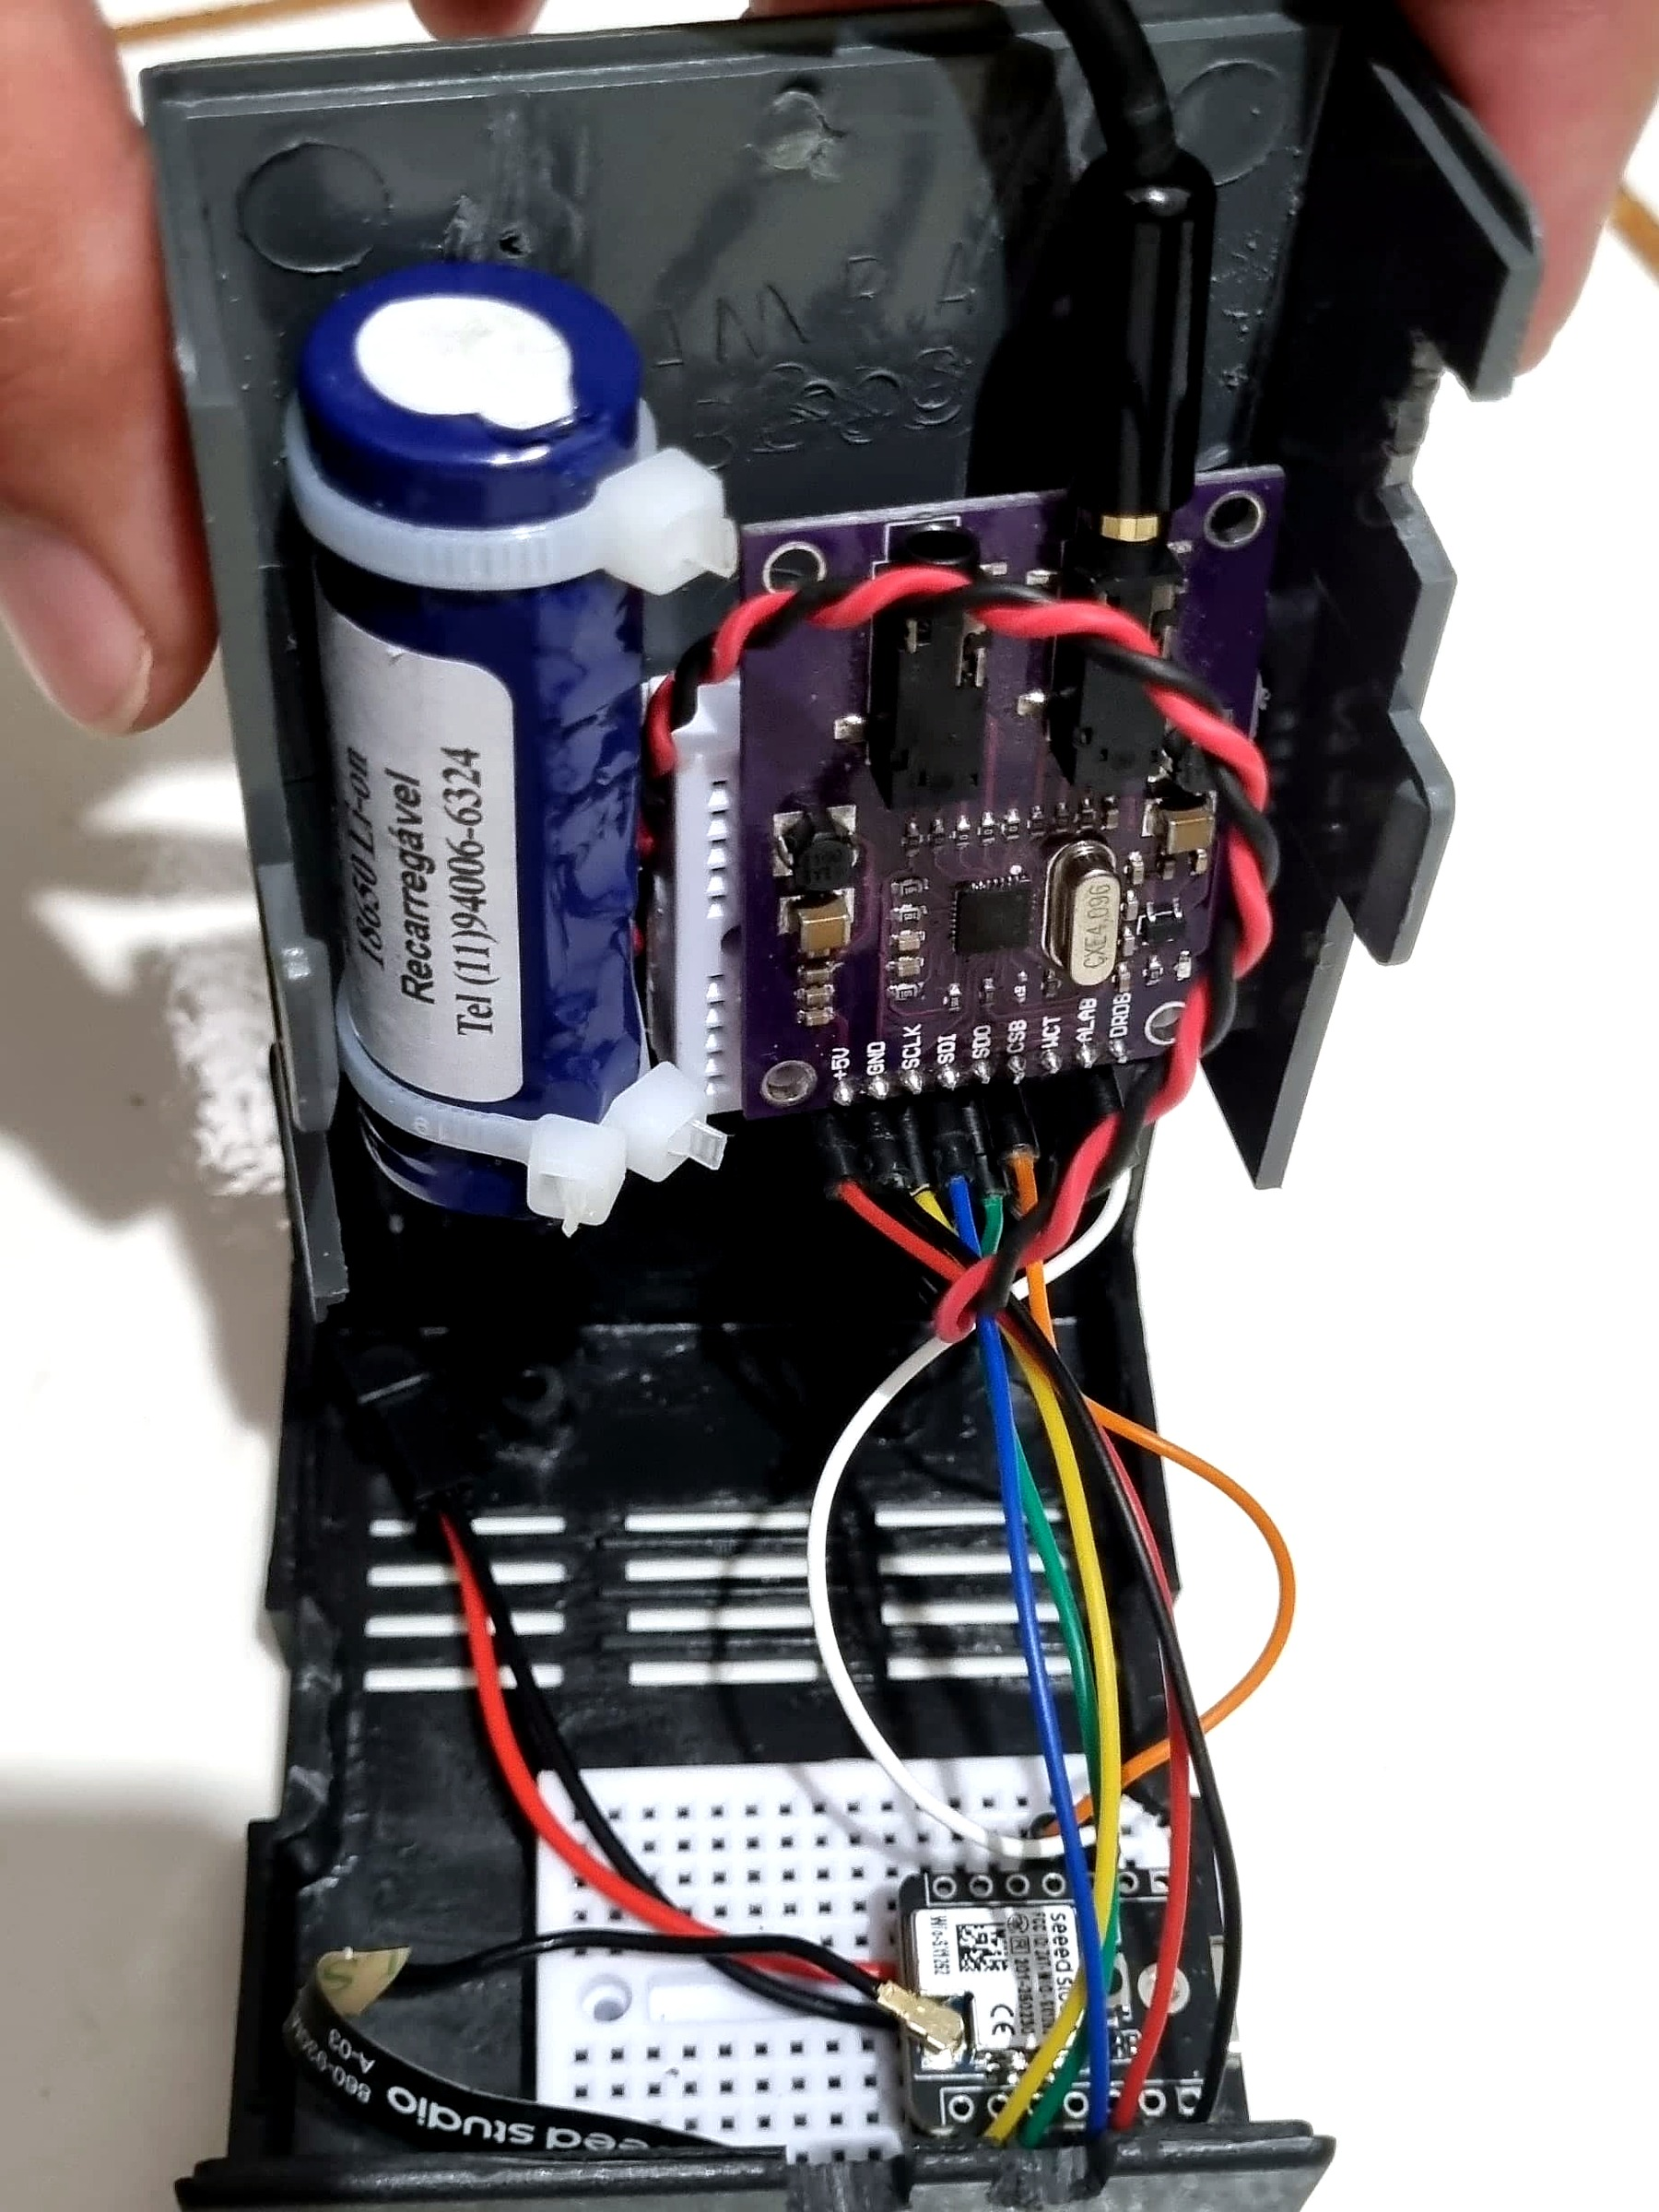
\includegraphics[width=0.30\linewidth]{assets/figura_03_prototipo_componentes_internos.jpg}}\hfill
\subfloat[Dispositivo montado e cabo de eletrodos]{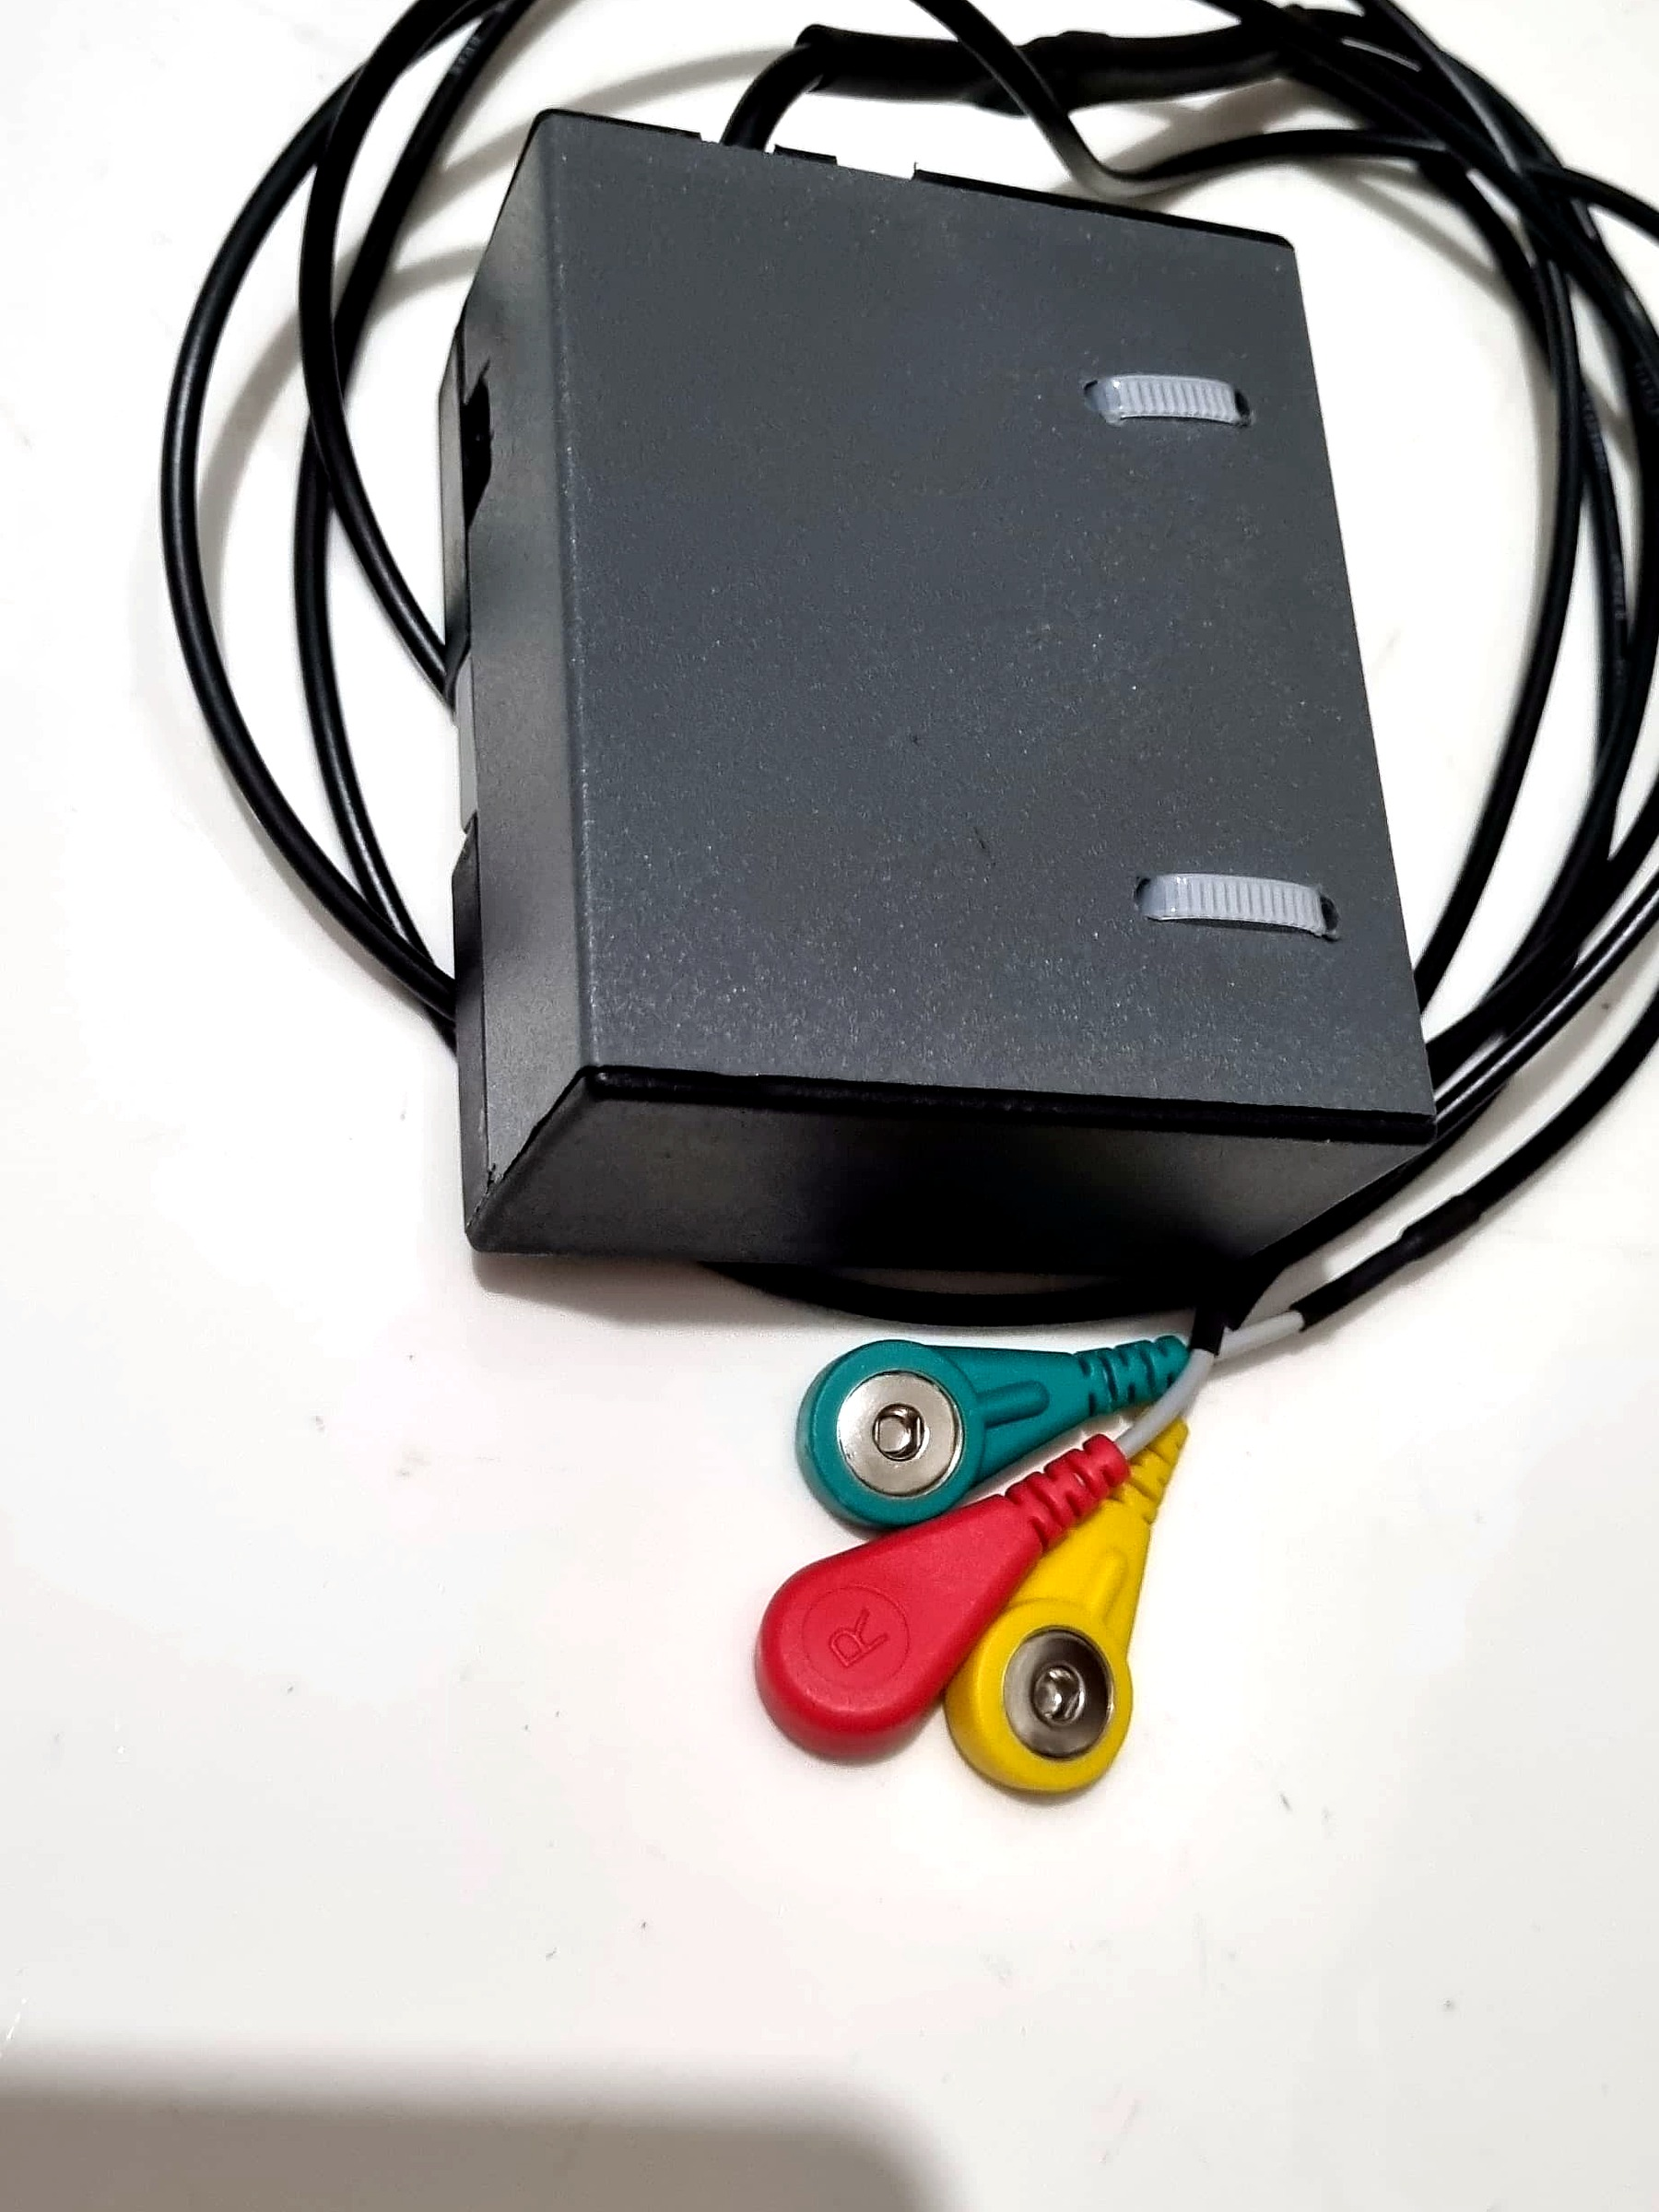
\includegraphics[width=0.30\linewidth]{assets/figura_01_prototipo_vista_superior_eletrodos.jpg}}\\[1ex]
\subfloat[Vista lateral: porta USB-C de recarga]{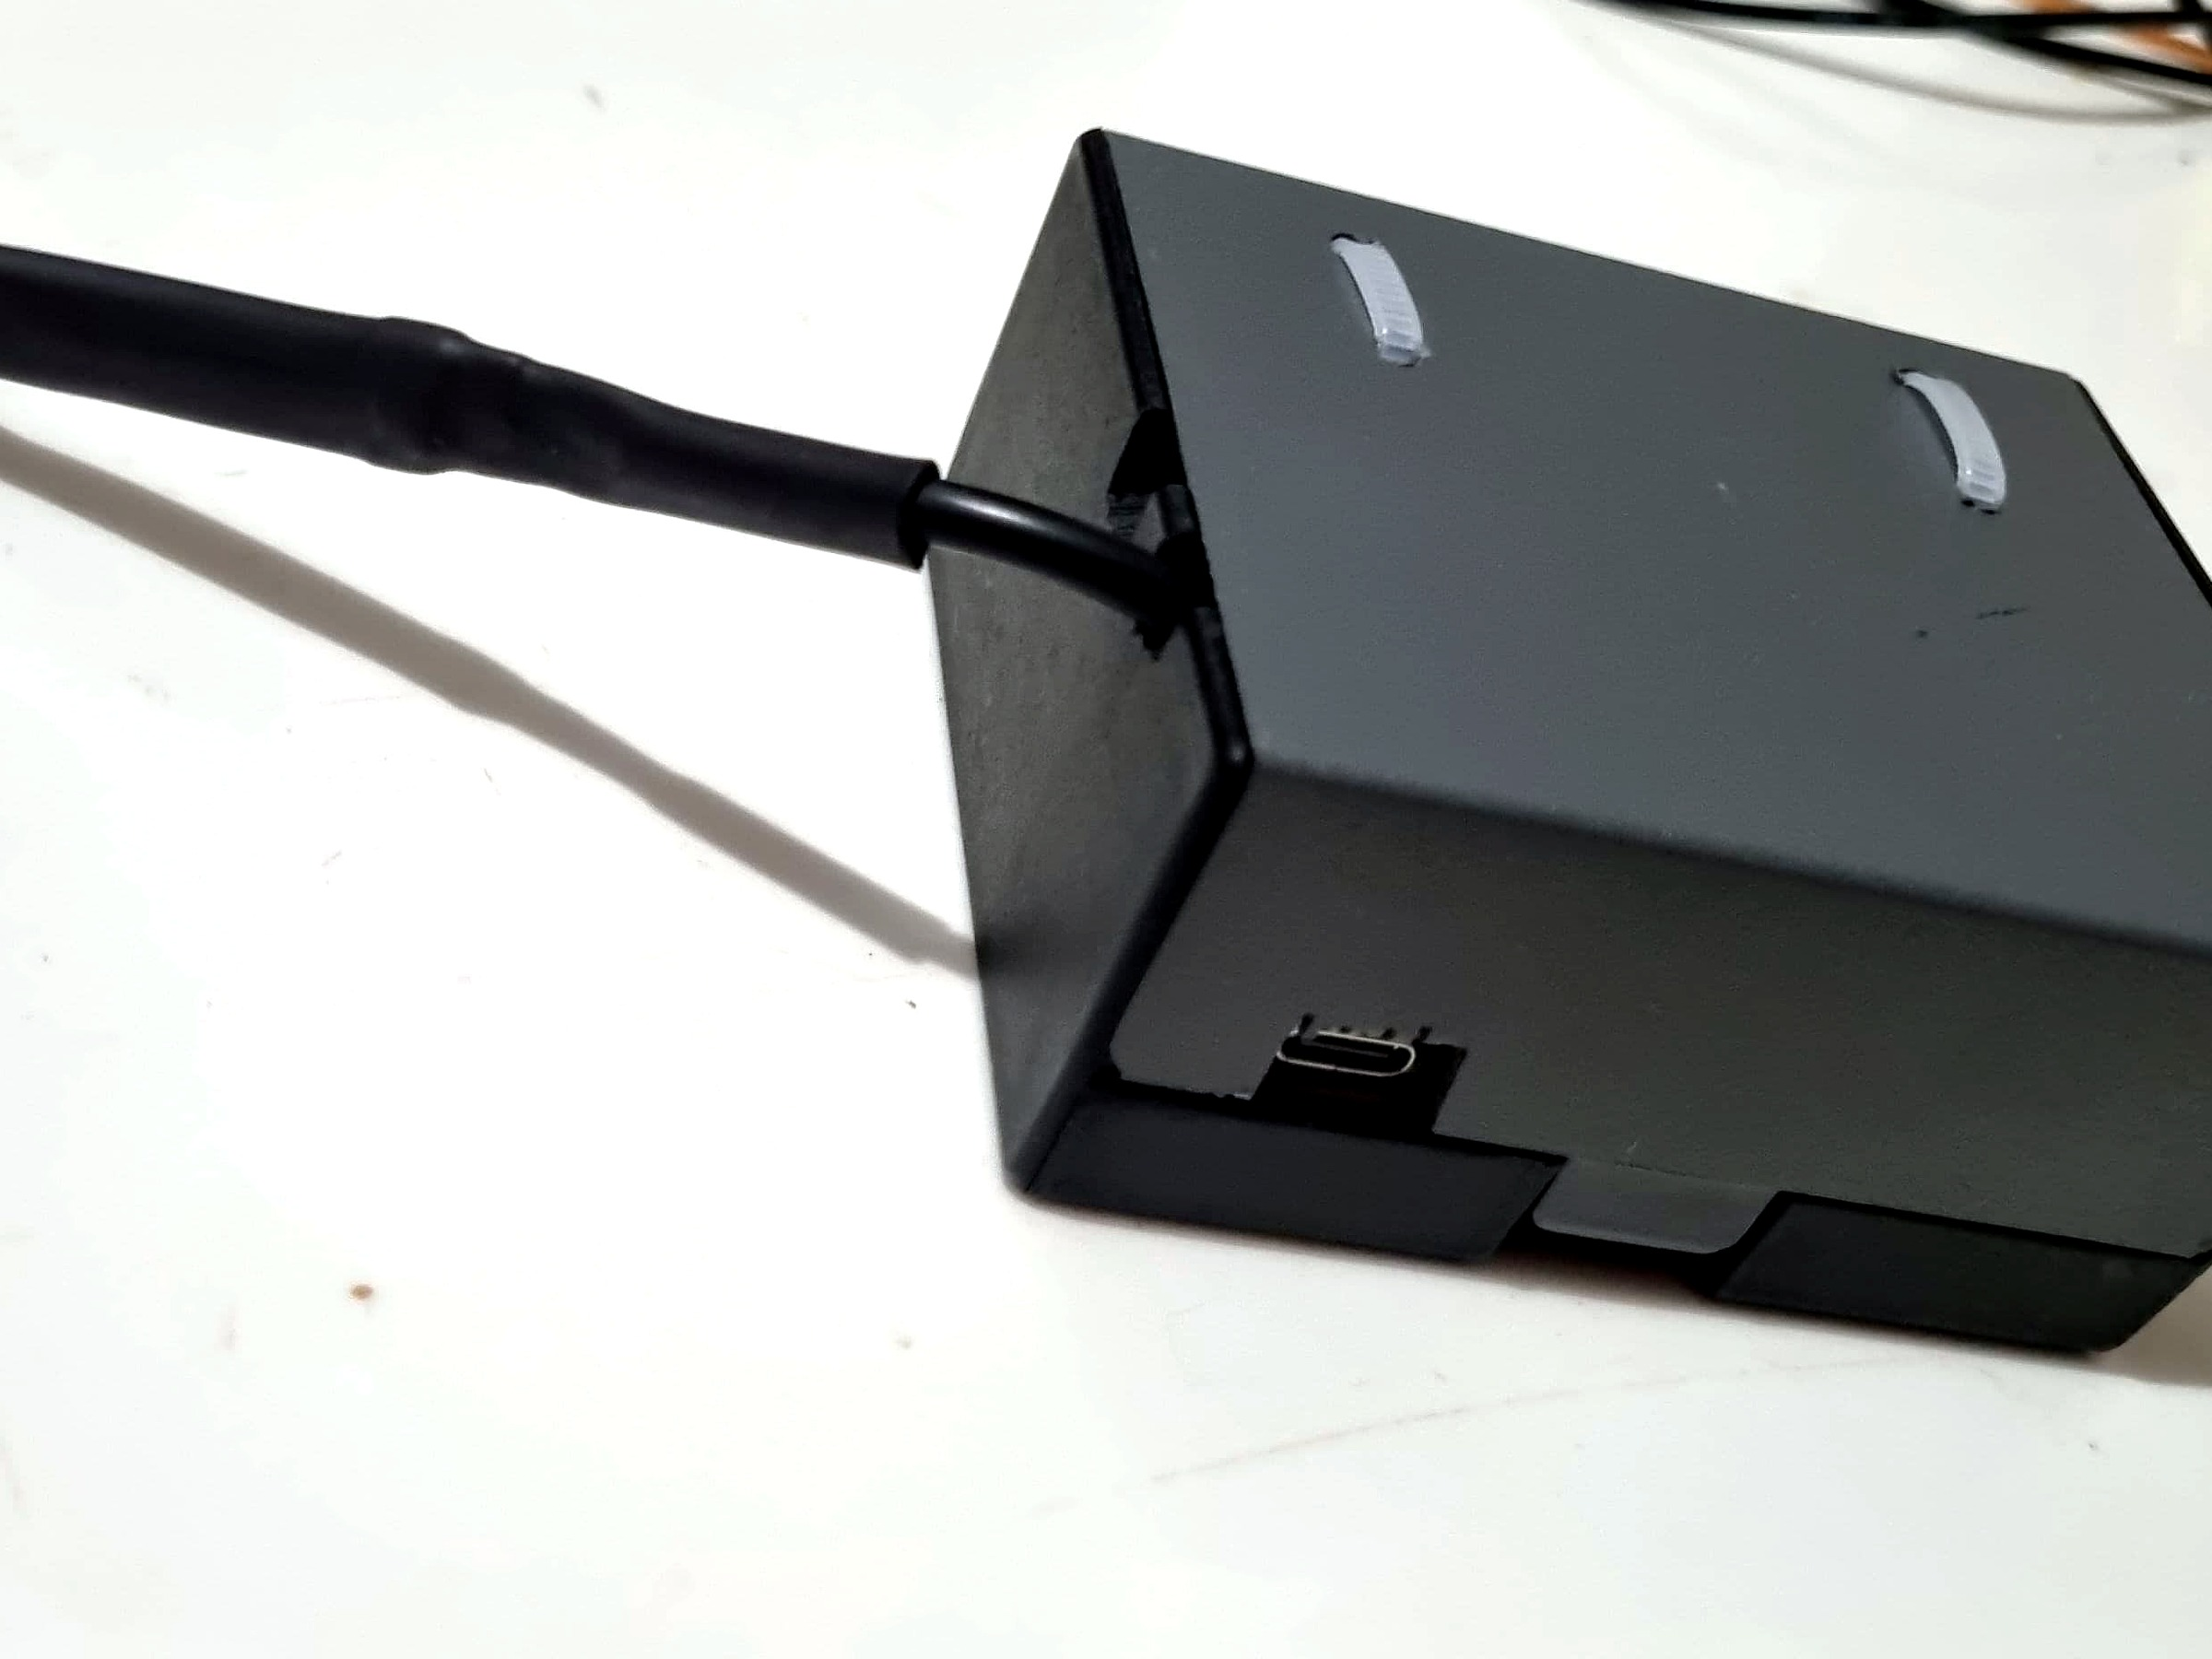
\includegraphics[width=0.55\linewidth]{assets/figura_02_prototipo_conector_usbc.jpg}}
\caption{Protótipo do dispositivo de aquisição de \acs{ECG}, encapsulado em caixa plástica comercial Patola\textsuperscript{\textregistered}, modelo PB-44: (a) vista interna, com a bateria de íons de lítio 18650 presa por abraçadeiras de náilon, a placa do \acs{AFE} CJMCU-1293 e, na base, o XIAO ESP32-S3 com o módulo Wio-SX1262 sobre matriz de contatos; (b) caixa fechada, com o cabo de três derivações e os eletrodos de pressão (\textit{snap}) nas cores do padrão IEC; (c) vista lateral, com o recorte da porta USB-C e a passagem do cabo de derivações.}
\label{fig:prototipo}
\end{figure}

\section{Desenvolvimento do Firmware Embarcado}
\label{sec:resFirmware}

O \textit{firmware} foi desenvolvido e encontra-se funcional em todas as suas etapas de processamento. A aquisição orientada a interrupção, disparada pelo sinal \acs{DRDY}, mostrou-se estável na taxa efetiva de 640 SPS (Seção~\ref{sec:resTaxa}), com leitura simultânea das três derivações pelo barramento \acs{SPI}. A cadeia de filtros digitais \acs{IIR} e o algoritmo de detecção de eventos foram implementados e executados sobre segmentos de 30~s armazenados na memória \textit{PSRAM} do microcontrolador, recurso que viabilizou o processamento de 19.200 amostras por segmento sem comprometer a memória interna.

O subsistema de armazenamento local em \textit{LittleFS} foi validado: para cada segmento processado, o resumo de 16 bytes foi gravado no \textit{log} binário, e a forma de onda dos segmentos sinalizados como anormais foi persistida integralmente, com as políticas de rotação operando conforme projetado. Os comandos de inspeção pela interface serial (despejo do \textit{log}, listagem e leitura dos arquivos de sinal bruto) permitiram auditar o conteúdo gravado e compará-lo com os dados recebidos na nuvem. O módulo de transmissão \textit{LoRaWAN}, baseado na biblioteca \textit{RadioLib}, realizou a montagem do \textit{payload} de 10 bytes e o envio na porta de aplicação 2, com a aquisição prosseguindo de forma independente do estado da conexão de rádio.

\section{Configuração da Rede LoRaWAN e Transmissão de Dados}
\label{sec:resTransmissao}

Inicialmente, realizou-se a configuração do \textit{gateway} da \textit{Radioenge} conectado ao \textit{Raspberry Pi 3} e a integração de um módulo Wio-SX1262 acoplado a um microcontrolador XIAO ESP32-S3. Essa integração facilitou os testes iniciais, permitindo direcionar os esforços para a comunicação com os servidores \textit{LoRaWAN}.

As primeiras tentativas de comunicação foram realizadas com a \acs{TTN}. Apesar de sua infraestrutura acessível e bem documentada, surgiram problemas recorrentes, como a exibição intermitente do dispositivo como \textit{offline}, mesmo com o envio de \textit{uplinks} válidos, além de latência variável na resposta dos pacotes e dependência integral de conectividade com a internet. A plataforma também impõe restrições à taxa de envio de mensagens (\textit{duty cycle}), dificultando aplicações que demandam transmissões frequentes.

Frente a essas dificuldades, a adoção de um servidor local com o \textit{ChirpStack} mostrou-se mais eficaz. A instalação local proporcionou maior controle sobre os componentes da rede, incluindo a visualização dos \textit{uplinks} em tempo real, a personalização dos parâmetros de recepção e a integração direta, via \acs{MQTT}, com a camada de aplicação. Embora tenha exigido uma curva de aprendizado mais acentuada, sobretudo na configuração dos perfis \acs{OTAA} e no roteamento interno dos dados, o servidor local demonstrou desempenho superior em termos de estabilidade e previsibilidade da comunicação.

Persistiram, contudo, desafios relacionados à natureza do protocolo \textit{LoRaWAN} em Classe~A, utilizado neste trabalho. Nesse modo, a abertura das janelas de recepção depende da transmissão anterior, o que limita substancialmente a taxa de envio. Em um dos experimentos, conduzido ainda sob a hipótese de transmitir a forma de onda, buscou-se enviar 15.000 amostras de \acs{ECG} comprimidas em blocos; embora a meta inicial fosse o envio de pacotes a cada 200 milissegundos, observou-se, na prática, intervalos entre 2 e 3 segundos por pacote, resultando em um tempo total de transmissão de aproximadamente 392,2 segundos — valor incompatível com aplicações em tempo quase real. Esse resultado, alinhado às restrições reportadas na literatura \citep{lorawanWaveform, 3-lead}, evidenciou a inviabilidade de transmitir a forma de onda completa e motivou a adoção da estratégia de detecção na borda, discutida na Seção~\ref{sec:resDeteccao}.

A banda AU915 (sub-banda 2) foi mantida ao longo de todos os testes, e o módulo Wio-SX1262 demonstrou compatibilidade e bom desempenho dentro das limitações do protocolo.

\section{Determinação da Taxa de Amostragem Efetiva}
\label{sec:resTaxa}

Durante a caracterização do ADS1293, constatou-se que a taxa de amostragem efetiva não correspondia ao valor anunciado pela biblioteca de controle. A configuração adotada é identificada na biblioteca como \texttt{SPS\_256} e ali documentada como 256 amostras por segundo\footnote{\textit{ProtoCentral ADS1293 ECG Library}, versão 1.3.0, de Protocentral Electronics, disponível em \url{https://github.com/Protocentral/protocentral-ads1293-arduino}. No arquivo \texttt{src/protocentral\_ads1293.h}, o comentário que acompanha a constante registra \texttt{SPS\_256, // R1=4, R2=5, R3=8 -> 102400/(4*5*8) = 256}: os fatores de decimação estão corretos, mas o quociente indicado não corresponde a eles.}. A contagem de amostras adquiridas no modo de diagnóstico do \textit{firmware}, contudo, indicou aproximadamente 1.920 amostras em 3~s, ou seja, cerca de 640 amostras por segundo --- duas vezes e meia o valor anunciado. A divergência importava porque os coeficientes dos filtros digitais e a conversão de amostras em tempo, da qual dependem os intervalos R-R, são calculados a partir dessa taxa.

Verificou-se, em seguida, qual das duas informações estava correta, recorrendo à cadeia de divisores do próprio conversor. Com a frequência de \textit{clock} interna $f_{CLK} = 409{,}6$~kHz, a frequência de modulação resulta em $f_{MOD} = f_{CLK}/4 = 102{,}4$~kHz, e a taxa de saída (\textit{Output Data Rate}) é dada pela Equação~\ref{eq:odr}:

\begin{equation}
    \text{ODR} = \frac{f_{MOD}}{R_1 \cdot R_2 \cdot R_3} = \frac{102{,}4 \times 10^3}{4 \cdot 5 \cdot 8} = 640 \text{ SPS}
    \label{eq:odr}
\end{equation}

\noindent em que $R_1$, $R_2$ e $R_3$ são os fatores de decimação configurados nos registradores do ADS1293. Os valores $R_1 = 4$, $R_2 = 5$ e $R_3 = 8$ são exatamente os que a biblioteca programa na configuração \texttt{SPS\_256}; aplicados à equação do manual do componente, resultam em 640~SPS, e não em 256. A divergência está, portanto, na nomenclatura e na documentação da biblioteca, e não entre teoria e medida: o valor calculado a partir dos registradores efetivamente programados coincide com o medido, e ambos estabelecem a taxa de amostragem efetiva do sistema em 640~SPS. Adotou-se esse valor em todo o processamento subsequente; mantida a taxa nominal de 256~SPS, as frequências de corte dos filtros e as estimativas de frequência cardíaca ficariam deslocadas pelo mesmo fator de 2,5.

\section{Aquisição do ECG Registrado no Próprio Autor}
\label{sec:resEcgProprio}

A primeira verificação da cadeia de aquisição foi feita sobre \acs{ECG} humano, registrado
no próprio autor. Ela não produz métrica de desempenho --- não há anotação de referência, e
o sujeito é um único indivíduo saudável ---, mas foi a etapa que revelou os dois defeitos
de aquisição corrigidos no trabalho e a limitação de especificidade do critério de arritmia
sinusal. Os traçados registrados não são reproduzidos neste texto: por se tratar de sinal
fisiológico humano, sua divulgação depende de apreciação por comitê de ética em pesquisa, à
qual o trabalho ainda não foi submetido. Relatam-se, portanto, apenas as grandezas
agregadas deles derivadas.

\subsection{Ausência de referência de modo comum e correção do acionamento de perna}
\label{sec:resSinal}

A aquisição do sinal foi avaliada por meio de uma ferramenta de visualização que recebe as três derivações pela interface serial do dispositivo. Nos ensaios preliminares, com o cabo de eletrodos posicionado segundo o triângulo de \textit{Einthoven}, o sinal capturado apresentou uma flutuação de baixa amplitude e frequência, sem as deflexões características do complexo QRS, da onda P e da onda T. Em consequência, o algoritmo de detecção não identificou picos R consistentes, sinalizando a maior parte dos segmentos como erro de processamento.

A investigação atribuiu o fenômeno à ausência de uma referência de modo comum efetiva: o amplificador de perna direita (\textit{Right-Leg Drive} -- RLD), necessário para estabilizar o potencial do corpo em relação ao circuito de entrada, não estava adequadamente conectado, deixando as entradas diferenciais sujeitas a interferência de modo comum. Como medida corretiva, adotou-se a configuração de \textit{driven-leg} de três eletrodos descrita na Seção~\ref{sec:cjmcu}, na qual a detecção de modo comum é realizada sobre os eletrodos RA e LL (\texttt{CMDET\_EN = 0x05}) e a contrarreação é reinjetada pelo eletrodo LA (\texttt{SELRLD = 010}).

A revalidação foi conduzida em um teste de bancada com o sistema conectado ao próprio autor. Registraram-se 30~s do sinal bruto de cada derivação, em modo de diagnóstico, sem filtragem. Nesse modo o \textit{firmware} imprime as três derivações a cada amostra, o que excede a capacidade do enlace serial (Seção~\ref{sec:resSerial}); por isso a ferramenta externa gravou 17.888 amostras no intervalo de 30~s --- cerca de 596 por segundo ---, e não as 19.200 que correspondem à taxa de conversão. A taxa do conversor é fixa em 640~SPS, imposta pelos divisores internos do ADS1293 (Seção~\ref{sec:resTaxa}); o que se reduz é o número de amostras que chegam ao computador, não a cadência com que o conversor as produz. Como a verificação se destinava à morfologia do traçado, e não à sua temporização, a perda não compromete a conclusão; a estimativa de frequência cardíaca dela derivada é, por essa razão, aproximada. Após a correção, a derivação II passou a exibir os complexos QRS de forma nítida e com a polaridade esperada, além das ondas P e T, permitindo a estimativa de uma frequência cardíaca em torno de 90~bpm.


Para quantificar o efeito do RLD sobre a interferência da rede elétrica, o teste foi repetido sob duas condições --- RLD ativo e RLD desconectado (\texttt{SELRLD = 000}) ---, mantendo-se inalterados os eletrodos, o seu posicionamento e o ambiente. Estimou-se, por análise espectral, a fração da energia total do sinal concentrada em torno de 60~Hz. Na derivação II, da qual o detector extrai os intervalos R-R, essa fração caiu de 0,081\,\% com o RLD desconectado para 0,019\,\% com o RLD ativo, redução de 4,3 vezes. Em valor absoluto, o valor eficaz da componente de 60~Hz passou de 0,0097 para 0,0053~mV, redução de 1,8 vezes --- a diferença entre as duas razões decorre de a energia total do sinal não ser idêntica nas duas aquisições. A Figura~\ref{fig:espectroRld} apresenta os dois espectros. Duas ressalvas delimitam o alcance da medida. Mesmo sem o RLD a energia de 60~Hz já era baixa, o que indica um ambiente eletromagneticamente favorável no ensaio; em instalações mais ruidosas espera-se benefício proporcionalmente maior do circuito. E trata-se de uma única aquisição de 30~s por condição, em um único ambiente: o valor quantifica o efeito observado nesta bancada, não uma figura de mérito do sistema.

\begin{figure}[htb]
\centering
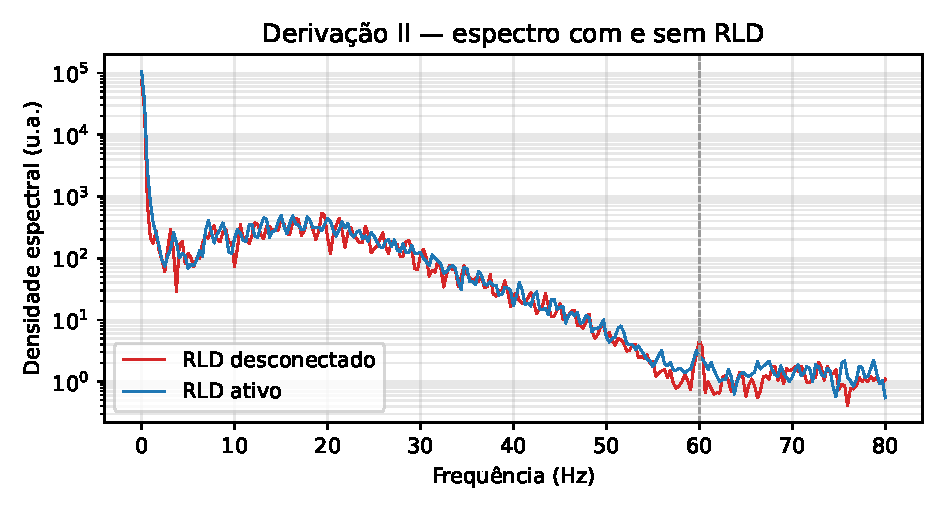
\includegraphics[width=0.9\textwidth]{assets/espectro_rld.pdf}
\caption{Espectro da derivação II no teste de bancada, com o RLD desconectado e ativo, estimado à taxa de amostragem do conversor (640~SPS). A linha tracejada indica a frequência da rede elétrica (60~Hz).}
\label{fig:espectroRld}
\end{figure}

Cabe destacar que a cadeia de condicionamento digital — composta pelos filtros passa-baixas (40~Hz) e passa-altas (0,5~Hz) descritos na Seção~\ref{sec:condicionamento} — foi assim avaliada sobre um sinal fisiológico real de boa qualidade, confirmando a remoção do desvio de linha de base e a preservação do complexo QRS de interesse.


\subsection{Especificidade do critério de arritmia sinusal em repouso}
\label{sec:resArritmia}

Além da validação da aquisição do sinal (Seção~\ref{sec:resSinal}), o algoritmo de detecção foi avaliado em um teste de bancada preliminar, com o sistema conectado ao próprio autor e a detecção ativa sobre segmentos de 30~s. Registraram-se sessões em duas posturas — em decúbito dorsal (repouso) e sentado. Os detectores de eventos clinicamente críticos — taquicardia, bradicardia, bloqueio e parada sinoatrial — não produziram falsos positivos em nenhuma das sessões. O detector de \textit{arritmia sinusal}, entretanto, sinalizou praticamente todos os segmentos.

A causa foi identificada no critério de decisão: o algoritmo marca o segmento como arritmia quando ocorre ao menos uma variação batimento-a-batimento do intervalo R-R superior a 120~ms. Em repouso, a arritmia sinusal respiratória — variação fisiológica e benigna do ritmo com a respiração, mediada pela modulação vagal do nó sinusal e acentuada pelo predomínio parassimpático nessa condição (\citeay{hrvTaskForce1996}; \citeay{guyton2021fisiologia}) — produziu, nas coletas desta bancada, cerca de 8 a 15 dessas variações por segmento de 30~s, de modo que o critério dispara em todos os segmentos. A rejeição dos batimentos eventualmente não detectados (intervalos R-R próximos ao dobro da mediana) removeu apenas uma fração das ocorrências, confirmando que a maior parte da variabilidade é de origem fisiológica.

A Tabela~\ref{tab:arritmiaPostura} resume a comparação entre as posturas. A frequência cardíaca elevou-se de cerca de 67~bpm, em repouso, para cerca de 92~bpm, na posição sentada, evidenciando que a aquisição acompanha corretamente a resposta autonômica; a taxa de segmentos sinalizados como arritmia, contudo, permaneceu elevada em ambas as condições, indicando que a manipulação postural não altera a especificidade do critério.

\begin{table}[htb]
\centering
\caption{Avaliação preliminar do detector de arritmia sinusal em duas posturas (teste de bancada, segmentos de 30~s).}
\label{tab:arritmiaPostura}
\begin{tabular}{l c c c}
\hline
\textbf{Condição} & \textbf{FC média} & \textbf{Variações R-R $>$120~ms} & \textbf{Segmentos} \\
                  & \textbf{(bpm)}    & \textbf{por segmento (média)}    & \textbf{sinalizados} \\
\hline
Decúbito (repouso) & $\approx$67 & $\approx$7,8 & 100\,\% \\
Sentado            & $\approx$92 & $\approx$8,6 & 100\,\% \\
\hline
\end{tabular}
\end{table}

Conclui-se que o critério de detecção de arritmia sinusal baseado na variabilidade do intervalo R-R apresenta especificidade intrinsecamente baixa para indivíduos saudáveis, uma vez que a arritmia sinusal respiratória constitui, ela própria, uma variação sinusal do ritmo. Trata-se de uma limitação conhecida da abordagem, e não de uma falha, portanto, a arritmia sinusal passou a ser tratada como informação de contexto, e não como alerta crítico, preservando-se como eventos críticos a taquicardia, a bradicardia e as pausas (bloqueio e parada sinoatrial), cuja detecção se mostrou específica. A caracterização quantitativa de sensibilidade e especificidade dessa e das demais classes, sobre sinais de classe conhecida, é apresentada nas Seções~\ref{sec:resEcgSintetico} e~\ref{sec:resEcgOrientadorFinal}, e sua generalização sobre a base anotada MIT-BIH, na Seção~\ref{sec:resMITBIH}.

Como medida de mitigação dessa limitação no nível da aplicação — sem alterar o critério de detecção na borda —, o aplicativo passou a exigir a confirmação por persistência antes de promover uma anomalia a alarme (Seção~\ref{sec:appFunc}). Os limiares padrão por classe constam da Tabela~\ref{tab:alarmePadrao}: a arritmia sinusal, por seu caráter fisiológico e recorrente, exige detecção em todos os dez últimos segmentos --- cerca de 5 minutos de persistência ---, ao passo que a parada sinoatrial alarma com uma única detecção. Dessa forma, reduz-se a taxa de alarmes falsos apresentada ao profissional, preservando-se integralmente o registro de todos os segmentos para análise posterior.

\section{Ensaios com ECG Sintetizado neste Trabalho}
\label{sec:resEcgSintetico}

Caracterizada a aquisição sobre \acs{ECG} humano, passou-se aos ensaios com \acs{ECG} de
classe conhecida, injetado na entrada do dispositivo pelo gerador de sinais descrito na
Seção~\ref{sec:validacaoGerador}. Os primeiros foram conduzidos sobre \acs{ECG} sintetizado
neste trabalho, escolha que tem uma razão de método: com o ritmo sob controle, qualquer
discrepância entre a classe esperada e a detectada só pode vir da cadeia de aquisição ou do
critério de decisão, e não do material de teste. Foi assim que se localizou o segundo
defeito de aquisição do trabalho.

\subsection{Saturação do enlace serial}
\label{sec:resSerial}

O primeiro dos dois defeitos foi identificado e corrigido durante estes ensaios com \acs{ECG} injetado de amplitude controlada. Constatou-se que a impressão contínua das três derivações pela interface serial, quando lida simultaneamente por uma ferramenta externa, exigia do enlace uma vazão superior à sua capacidade — cerca de 270~kbit/s contra os 230.400 bits por segundo configurados (Seção~\ref{sec:condicionamento}). Excedida a capacidade, a escrita bloqueava momentaneamente o laço de aquisição, reduzindo a taxa efetivamente registrada de 640 para cerca de 560 amostras por segundo. As amostras perdidas introduziam descontinuidades no \textit{buffer} que encurtavam artificialmente parte dos intervalos R-R e faziam o critério de variabilidade sinalizar arritmia de modo indevido, ainda que o sinal injetado fosse um ritmo regular. Ao desacoplar a saída de depuração da aquisição, por meio da decimação da impressão serial (Seção~\ref{sec:condicionamento}), o \textit{buffer} voltou a receber a totalidade das amostras: para um mesmo sinal normal injetado, os segmentos passaram a ser classificados corretamente como normais de forma consistente.

\subsection{Perda periódica de amostras na aquisição}
\label{sec:resPerdaAmostras}

Corrigida a saturação do enlace, restou um sintoma mais discreto: segmentos de ritmo normal continuavam a ser sinalizados como arritmia sinusal, de forma recorrente e sem que o \acs{ECG} injetado contivesse qualquer irregularidade. Duas hipóteses foram levantadas antes de se chegar à causa. A primeira atribuía o problema à frequência cardíaca do \acs{ECG} normal exatamente igual ao limiar: o traçado normal de 60~bpm possui R-R de exatamente 1000~ms, coincidente com o limiar de bradicardia, com margem nula; a adoção de um \acs{ECG} de 75~bpm (R-R de 800~ms, 200~ms de margem) eliminou as marcações indevidas de bradicardia, mas não as de arritmia. A segunda atribuía o problema à descontinuidade entre segmentos (Seção~\ref{sec:resProcedimento}), que a reprodução em laço introduz na junção entre o fim e o início do arquivo — como o arquivo tinha 30~s e o segmento de processamento também, ocorreria uma descontinuidade entre o final de um segmento gerado e o início do próximo; geraram-se então arquivos de 300~s, mas a hipótese foi refutada, pois 24 dos 30 segmentos continuaram a ser classificados erroneamente.

Esse resultado motivou o registro do sinal bruto adquirido. No traçado bruto (Figura~\ref{fig:perdaAmostras}), identificaram-se seis intervalos R-R anômalos, periódicos a cada aproximadamente 4,9~s, cada um com o intervalo de 800~ms reduzido para cerca de 710~ms. A causa foi localizada na aquisição, em um mecanismo distinto do da saturação serial (Seção~\ref{sec:resSerial}): agora com a saída de depuração já decimada, era a própria rotina de diagnóstico que consultava o espaço ocupado no sistema de arquivos local (\textit{LittleFS}) dentro do laço principal, a cada 5~s, bloqueando o processador por cerca de 105~ms; como a rotina de interrupção apenas sinaliza a disponibilidade de uma nova amostra, cerca de 66 amostras eram perdidas. O relatório de diagnóstico registrava 3.133 amostras válidas em vez das 3.200 esperadas — uma perda de 2,08\,\%, mais sutil que a da saturação serial (que reduzia a taxa a cerca de 560~SPS) e, por isso mesmo, mais difícil de identificar.

Ambos os problemas decorrem da mesma decisão de projeto: a rotina de interrupção associada ao sinal \acs{DRDY} apenas sinaliza a disponibilidade de uma nova amostra, e a leitura pelo barramento \acs{SPI} ocorre no laço principal. Nesse arranjo, a integridade da aquisição depende de o laço nunca bloquear por mais de um período de amostragem (1,56~ms a 640~SPS) --- condição silenciosamente violada pelas duas rotinas identificadas. O arranjo mais robusto é outro: executar a leitura do conversor dentro da própria rotina de interrupção, com prioridade máxima, gravando a amostra em memória antes de retornar; nesse caso, um bloqueio no laço atrasa o processamento, mas não descarta amostra alguma. Ele não foi adotado porque a leitura do \acs{AFE} é feita pela biblioteca de controle de terceiros empregada, cujas transações \acs{SPI} recorrem à interface padrão do \textit{framework} e não satisfazem os requisitos de execução em contexto de interrupção do ESP32, que exige que o código chamado resida na memória interna de instruções. Reescrever esse caminho implicaria substituir a biblioteca. Optou-se, em vez disso, por remover do laço as chamadas bloqueantes e por instrumentar a aquisição: o contador de interrupções \acs{DRDY} passou a ser comparado ao de leituras efetivadas, e a diferença entre ambos --- as amostras perdidas --- passou a constar do relatório de diagnóstico. Sob essa instrumentação, os ensaios subsequentes transcorreram sem perda registrada. A migração da leitura para a rotina de interrupção permanece como melhoria recomendada, por eliminar a falha por construção, e não por vigilância.

\begin{figure}[htbp]
\centering
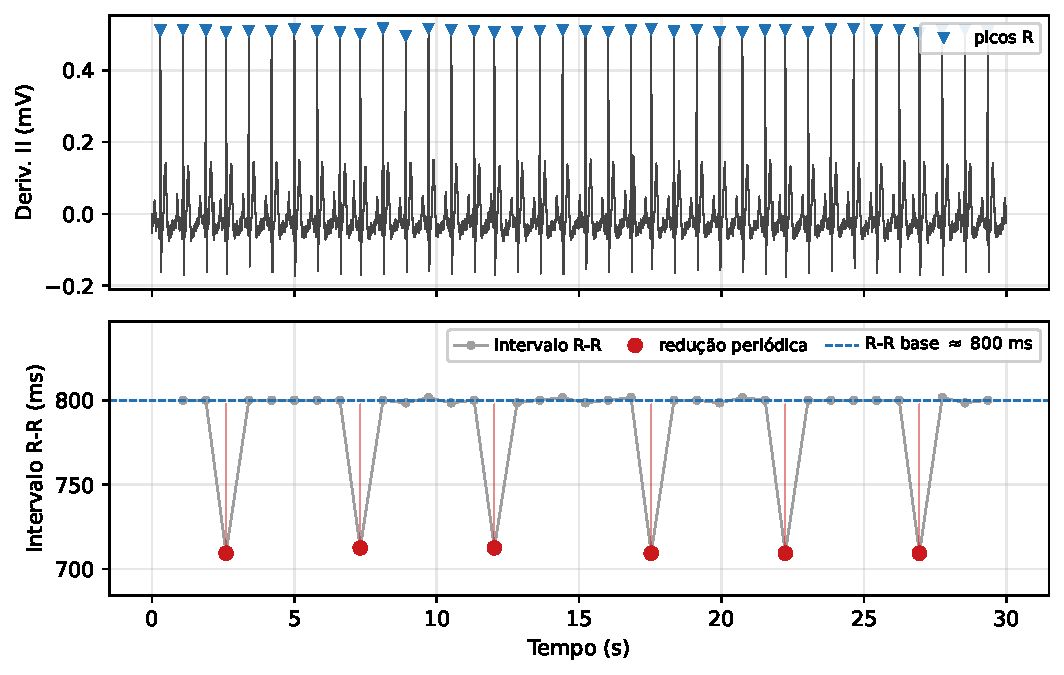
\includegraphics[width=0.95\linewidth]{assets/perda_amostras_rr.pdf}
\caption{Perda de amostras no sinal bruto de um segmento normal (75~bpm) indevidamente classificado como arritmia. Acima, a derivação II adquirida, com os picos R detectados; abaixo, a série de intervalos R-R, na qual se observam seis reduções periódicas — de $\approx$800 para $\approx$710~ms, a cada $\approx$4,9~s —, coincidentes com o bloqueio do laço de aquisição pela rotina de diagnóstico.}
\label{fig:perdaAmostras}
\end{figure}

Esse problema explicava todos os sintomas observados: a estimativa de frequência cardíaca cerca de 2\,\% maior; a aparente taxa de amostragem de 627~SPS, quando a taxa efetiva é de 640~SPS (Seção~\ref{sec:resTaxa}); e as marcações indevidas de arritmia, pois a diminuição periódica produzia variações R-R de 89 a 114~ms, muito próximas do limiar de 120~ms. A correção consistiu em remover do laço de aquisição a consulta ao sistema de arquivos.

\subsection{Desempenho sobre o ECG sintetizado e alcance do resultado}
\label{sec:resBateriaControlada}

Corrigida a aquisição, o ensaio foi repetido sobre um \acs{ECG} sintetizado de ritmo
estritamente controlado --- batimento obtido por soma de gaussianas, amplitude constante e
intervalos R-R distantes dos limiares de decisão ---, com 30 segmentos por classe e 180
ensaios no total. Os 180 segmentos foram classificados corretamente. O traçado normal, que
antes da correção era reconhecido em 20\,\% dos segmentos, passou a 100\,\%.

Esse resultado, entretanto, deve ser lido com três ressalvas, todas decorrentes do próprio
controle que o torna útil. O \acs{ECG} era sintético e de amplitude constante, e portanto
não exercitava o limiar global de amplitude do detector. Os intervalos R-R situavam-se
distantes dos limiares de decisão, o que dispensava a estimativa de qualquer precisão. E
cada intervalo R-R correspondia a um número inteiro de amostras --- 800~ms equivalem a
exatamente 512 amostras a 640~SPS ---, de modo que a quantização do instante do pico não
introduzia erro algum na estimativa da frequência cardíaca. Trata-se, portanto, do limite
superior do desempenho, obtido em condições deliberadamente favoráveis.

Para afastar as duas primeiras ressalvas sem perder o controle sobre o ritmo, sintetizou-se
um segundo conjunto, que adota como molde morfológico o batimento do \acs{ECG} cedido pelo
orientador e lhe impõe ritmo próprio: intervalo R-R de 800~ms (75~bpm) no traçado normal,
500~ms (120~bpm) na taquicardia e 1.200~ms (50~bpm) na bradicardia, com variabilidade
batimento a batimento de desvio-padrão de 15, 10 e 20~ms, respectivamente --- valores bem
abaixo do limiar de 120~ms do critério de arritmia sinusal, para não induzir classe falsa.
Sobre esse ritmo somaram-se imperfeições de amplitude, todas referidas à amplitude da onda
R: deriva senoidal de linha de base de 5\,\%, modulação respiratória de $\pm$8\,\% e ruído
branco de desvio-padrão de 2\,\%. Cabe registrar que apenas a \emph{morfologia} do batimento
provém do material externo; o ritmo e as pausas foram gerados aqui, de modo que as
limitações de ritmo do conjunto original, discutidas na Seção~\ref{sec:resModificacoes}, não
se transferem para este \acs{ECG}.

Sobre esse segundo conjunto, o sistema novamente classificou corretamente os 180 segmentos
(Tabela~\ref{tab:matrizFinal}), com as métricas por classe da
Tabela~\ref{tab:metricasClasse} e nenhum erro de processamento, o que indica integridade da
aquisição ao longo de todos os ensaios.

Cabe uma precisão sobre o alcance desse resultado, que diz respeito à regra de decisão
então vigente. Estes ensaios foram conduzidos sob o critério de pausa por duração absoluta,
e o \acs{ECG} de bloqueio foi construído para satisfazê-lo, com pausas na faixa de 4 a 6~s.
Sobre um ritmo de base de 800~ms, essas pausas equivalem a mais de cinco ciclos cardíacos,
de modo que a formulação relativa adotada depois (Seção~\ref{sec:resCriterioPausa}) as
classifica como \emph{parada sinusal}, e não como bloqueio. Reprocessado o mesmo arquivo
sob a regra final, as janelas de 30~s saem, de fato, como parada. A observação não aponta
defeito de detecção: ilustra que o material de teste acompanha a definição do critério, e
que a pausa de um bloqueio não se caracteriza por durar um certo número de segundos, mas
por fechar um número inteiro de ciclos do ritmo que a precede. É o mesmo fenômeno que, em
sentido inverso, impedia o reconhecimento das pausas do \acs{ECG} cedido pelo orientador
(Seção~\ref{sec:resOrigLimpo}).

\begin{table}[htb]
\centering
\caption{Matriz de confusão dos ensaios sobre o \acs{ECG} sintetizado neste trabalho (30 segmentos por classe; linha = classe esperada, coluna = classe detectada).}
\label{tab:matrizFinal}
\begin{tabular}{l c c c c c c}
\hline
\textbf{Esperada / Detectada} & \textbf{Normal} & \textbf{Taqui.} & \textbf{Bradi.} & \textbf{Arrit.} & \textbf{Bloq.} & \textbf{Parada} \\
\hline
Normal            & 30 & 0  & 0  & 0  & 0  & 0  \\
Taquicardia       & 0  & 30 & 0  & 0  & 0  & 0  \\
Bradicardia       & 0  & 0  & 30 & 0  & 0  & 0  \\
Arritmia sinusal  & 0  & 0  & 0  & 30 & 0  & 0  \\
Bloqueio sinoatr. & 0  & 0  & 0  & 0  & 30 & 0  \\
Parada sinoatr.   & 0  & 0  & 0  & 0  & 0  & 30 \\
\hline
\end{tabular}
\end{table}

\begin{table}[htb]
\centering
\caption{Desempenho de detecção por classe sobre o \acs{ECG} sintetizado neste trabalho (valores em \%).}
\label{tab:metricasClasse}
\begin{tabular}{l c c c c c c}
\hline
\textbf{Classe} & \textbf{N} & \textbf{Sens.} & \textbf{Espec.} & \textbf{\acs{VPP}} & \textbf{\acs{VPN}} & \textbf{Taxa de acerto} \\
\hline
Normal            & 30 & 100,0 & 100,0 & 100,0 & 100,0 & 100,0 \\
Taquicardia       & 30 & 100,0 & 100,0 & 100,0 & 100,0 & 100,0 \\
Bradicardia       & 30 & 100,0 & 100,0 & 100,0 & 100,0 & 100,0 \\
Arritmia sinusal  & 30 & 100,0 & 100,0 & 100,0 & 100,0 & 100,0 \\
Bloqueio sinoatr. & 30 & 100,0 & 100,0 & 100,0 & 100,0 & 100,0 \\
Parada sinoatr.   & 30 & 100,0 & 100,0 & 100,0 & 100,0 & 100,0 \\
\hline
\end{tabular}
\end{table}

Diferentemente do ensaio anterior, o erro de estimativa da frequência cardíaca não foi nulo
(Tabela~\ref{tab:erroFC}), o que era esperado diante da variabilidade imposta aos intervalos
R-R. O erro absoluto médio permaneceu, ainda assim, abaixo de 0,5~bpm nas três classes de
ritmo regular, com erro máximo de 1~bpm --- margem confortável frente ao limite admitido
para medidores de frequência cardíaca, de $\pm$10\,\% da frequência de entrada ou
$\pm$5~bpm, prevalecendo o maior (AAMI, \citeyear{aamiEC13}); a exatidão do medidor de
frequência cardíaca é também objeto da norma particular dos equipamentos de monitorização
de \acs{ECG} (IEC, \citeyear{iec6060127}). As classes de arritmia e de pausa foram omitidas
desta análise por não possuírem frequência cardíaca regular ao longo de todo o segmento.

\begin{table}[htb]
\centering
\caption{Erro de estimativa da frequência cardíaca nas classes de ritmo regular, sobre o \acs{ECG} sintetizado neste trabalho (em bpm).}
\label{tab:erroFC}
\begin{tabular}{l c c c c}
\hline
\textbf{Classe} & \textbf{N} & \textbf{Erro médio abs.} & \textbf{Erro máx.} & \textbf{Desvio-padrão} \\
\hline
Normal      & 30 & 0,4 & 1,0 & 0,5 \\
Taquicardia & 30 & 0,2 & 1,0 & 0,4 \\
Bradicardia & 30 & 0,5 & 1,0 & 0,5 \\
\hline
\end{tabular}
\end{table}

Cabe uma ressalva final. O reconhecimento integral do \acs{ECG} normal nestes ensaios não
contradiz a baixa especificidade do critério de arritmia sinusal caracterizada na
Seção~\ref{sec:resArritmia}. O \acs{ECG} normal sintetizado possui variabilidade R-R
limitada --- variação inferior ao limiar de 120~ms ---, ao passo que o \acs{ECG} de um
indivíduo real em repouso exibe arritmia sinusal respiratória de amplitude suficiente para
satisfazer o critério. A limitação manifesta-se sobre sinal fisiológico humano, não sobre
\acs{ECG} controlado.

\section{Ensaios com o ECG Cedido pelo Orientador: Versão Original do Algoritmo}
\label{sec:resEcgOrientadorOriginal}

As duas etapas anteriores empregaram \acs{ECG} de origem própria --- registrado no autor ou
sintetizado aqui. Esta emprega material independente: seis arquivos de \acs{ECG} sintético,
um por classe, cedidos pelo orientador, com complexo P-QRS-T invariante ao longo do registro
e ritmo especificado por ele. A independência importa porque remove do autor a escolha do
material com que o seu próprio sistema é avaliado. Os ensaios desta seção foram conduzidos
sobre a \emph{versão original} do algoritmo de detecção, tal como cedido por seus autores,
e é por isso que eles expõem as limitações que a Seção~\ref{sec:resModificacoes} consolida.

\subsection{Desempenho sobre ECG sem ruído}
\label{sec:resOrigLimpo}

As quatro classes definidas pelo ritmo --- normal a 63~bpm, taquicardia a 105~bpm,
bradicardia a 57~bpm e arritmia sinusal com variação R-R de 130~ms --- foram reproduzidas
pelo gerador e processadas em 30 segmentos cada, totalizando 120 ensaios. Todos os 120 foram
classificados corretamente, sem erro de processamento, e o erro absoluto médio de estimativa
da frequência cardíaca foi nulo nas quatro classes. Esse erro nulo não é mérito do
estimador, e convém dizê-lo: o \acs{ECG} cedido é exatamente periódico, de modo que a
frequência de referência é um valor único e a estimativa o reproduz sem resíduo. A medida
representativa do erro sob ritmo variável é a da Seção~\ref{sec:resBateriaControlada}, entre
0,2 e 0,5~bpm.

As duas classes de pausa não puderam ser ensaiadas com os arquivos originais, e a razão é o
próprio critério então vigente. O algoritmo definia bloqueio e parada por \emph{duração
absoluta} da pausa: exigia ao menos duas pausas entre 4 e 6~s para o bloqueio sinoatrial, e
uma pausa acima de 6~s para a parada sinusal. As pausas dos arquivos cedidos foram
construídas, corretamente, como múltiplos do intervalo R-R de base --- 1.904~ms
($2\times$952) e 2.856~ms ($3\times$952) no bloqueio, 3.332~ms ($3{,}5\times$952) na parada
---, que é a representação fisiológica do quadro: no bloqueio sinoatrial de segundo grau o
impulso é barrado e a pausa fecha em número inteiro de ciclos. Nenhuma delas alcança o piso
de 4~s. Em ensaio prévio de duas repetições por classe, os segmentos saíram com máscara
\texttt{0x06} --- bradicardia acompanhada de arritmia --- e foram rotulados como
bradicardia, sem qualquer detecção de pausa. O resultado é determinístico, e não amostral:
decorre da comparação entre a duração das pausas do arquivo e o piso do critério, de modo
que repetir o ensaio 30 vezes produziria trinta vezes o mesmo desfecho. Optou-se por não
comprometer as horas de bancada para reproduzi-lo.

Para fechar as seis classes sob o critério absoluto, os dois \acs{ECG} de pausa foram
remontados com material do próprio arquivo cedido: como o \acs{ECG} dele é exatamente
periódico e tem linha de base nula, cada segmento foi montado como uma sequência de
posições de um ciclo, em que cada posição recebe ou um batimento recortado do seu arquivo
normal, ou um ciclo de silêncio. Nada foi sintetizado; alterou-se apenas quantos ciclos de
silêncio separam dois batimentos, de modo a produzir pausas de $5\times$R-R (4.760~ms) e de
$7\times$R-R (6.664~ms), que recaem dentro da faixa absoluta exigida. Sobre esses dois
\acs{ECG}, as duas classes de pausa foram reconhecidas nos 30 segmentos cada, com 60 ensaios
sem erro de processamento.

Cabe registrar a fragilidade dessa evidência, e ela é de princípio: um \acs{ECG} construído
por quem também escolhe o critério demonstra que a cadeia reproduz e classifica a pausa, não
que o detector reconheça pausas arbitrárias. O desfecho relevante desta etapa não é,
portanto, a taxa de acerto, mas a constatação que a precedeu --- o critério por duração
absoluta obrigava a distorcer o material de teste para que ele caiba na regra, em vez de
reconhecer o quadro clínico tal como ele se apresenta. Foi essa constatação que motivou a
revisão descrita na Seção~\ref{sec:resCriterioPausa}.

\subsection{Desempenho sob ruído somado}
\label{sec:resRuido}

Os ensaios anteriores empregaram \acs{ECG} livre de ruído, adequado para isolar o comportamento do detector frente ao ritmo, mas distante das condições de aquisição em campo. Para caracterizar a robustez do sistema a interferências, somou-se ruído sintético ao \acs{ECG} das seis classes, reproduzindo o ensaio conduzido por \citeay{moraesFirmwareECG}. Foram consideradas três perturbações --- uma senoide de 0,33~Hz, que simula a deriva da linha de base pela respiração; uma senoide de 60~Hz, que simula a interferência da rede elétrica; e um ruído aleatório de banda larga, que simula os artefatos de movimento e de atividade muscular ---, cada uma somada em três amplitudes, correspondentes a 10, 20 e 30\,\% da excursão pico-a-vale do sinal sem ruído. A combinação das seis classes com os três tipos de perturbação e as três amplitudes resultou em 54 condições distintas que, a 30 repetições cada, totalizaram 1.620 ensaios. Nenhum ensaio retornou erro de processamento.

A Figura~\ref{fig:ruidoTipos} ilustra os três tipos de perturbação, na maior amplitude, somados ao \acs{ECG} normal. A Tabela~\ref{tab:ruidoAcuracia} resume a taxa de acerto por condição. A taxa de acerto total foi de 93,5\,\% (1.515 dos 1.620 ensaios).

\begin{figure}[htbp]
\centering
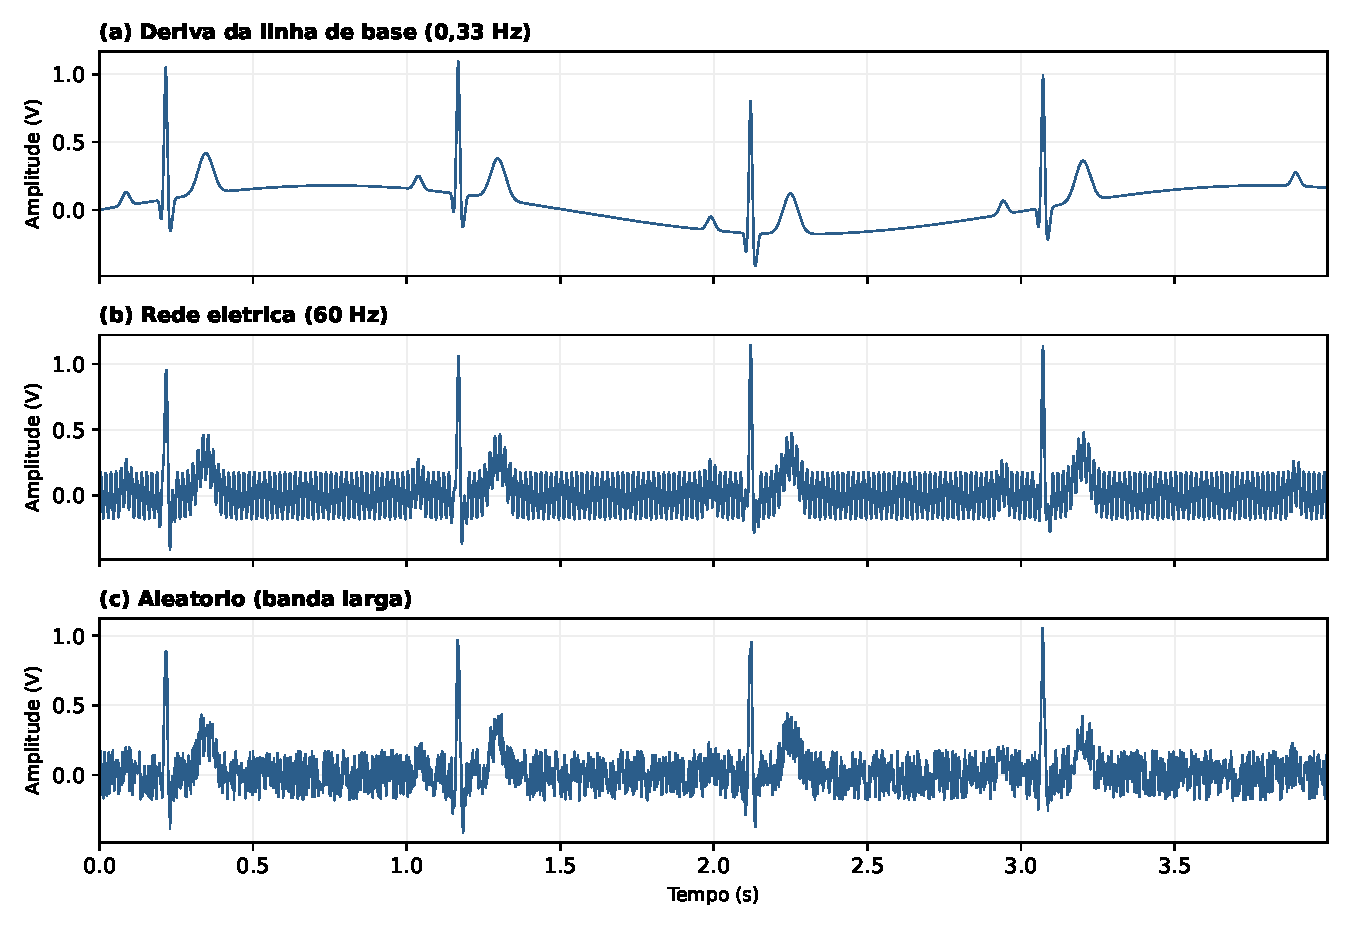
\includegraphics[width=\linewidth]{assets/figura_ruido_tipos.pdf}
\caption{\acs{ECG} normal com cada um dos três tipos de ruído somado a 30\,\% da excursão do sinal: (a) deriva da linha de base a 0,33~Hz; (b) interferência de rede a 60~Hz; (c) ruído aleatório de banda larga. Trecho de 4~s.}
\label{fig:ruidoTipos}
\end{figure}

A deriva de 0,33~Hz não produziu erro algum em nenhuma amplitude, resultado esperado, uma vez que sua frequência situa-se abaixo do corte do filtro passa-alta de 0,5~Hz do \textit{firmware} e é, portanto, atenuada antes da detecção. O ruído aleatório degradou o desempenho apenas na maior amplitude, e ainda assim de forma parcial (92,2\,\% a 30\,\%): a única classe afetada foi a normal, na qual a perturbação de banda larga ocasionalmente introduz um pico indesejado que eleva a variabilidade R-R acima do limiar de arritmia. Trata-se da mesma condição em que \citeay{moraesFirmwareECG} registraram o único resultado inconsistente do algoritmo original --- ruído aleatório na amplitude de 30\,\% ---, ainda que a manifestação difira: ali a taxa de acerto caiu a 98,33\,\% na detecção de bloqueio sinoatrial, com sensibilidade de 90\,\%, por \emph{perda} de picos R; aqui, a falha decorre da introdução de um pico \emph{indesejado} sobre o traçado normal. O que se repete, portanto, não é o desfecho, mas a natureza da limitação e o patamar em que ela se manifesta: a localização dos complexos pelo método da operação de diferenças degrada-se sob ruído de banda larga a partir de 30\,\% da excursão, amplitude que os próprios autores identificam como aquela em que o algoritmo "apresentou certa dificuldade na detecção dos picos R".

A divergência quanto à classe afetada encontra explicação no escopo distinto dos dois experimentos. Os ensaios de \citeay{moraesFirmwareECG} alimentaram o algoritmo diretamente com vetores de amostras produzidos por programa, aos quais o ruído fora somado --- de modo que a perturbação vista pelo detector é exatamente a especificada. Nos ensaios aqui relatados, o \acs{ECG} perturbado é reproduzido fisicamente e percorre o divisor resistivo, o \acs{AFE}, a quantização a 640~SPS e a cascata de filtros antes de alcançar o detector; o passa-baixas de 40~Hz remove parte da banda larga, ao passo que a cadeia analógica acrescenta seu próprio resíduo. O ruído que chega ao algoritmo não é, portanto, o mesmo, ainda que a especificação de amplitude o seja. As duas medidas não se contradizem: uma caracteriza o \emph{algoritmo} isoladamente, a outra o \emph{sistema} que o incorpora, e é a segunda que interessa ao propósito desta dissertação.

\begin{table}[htb]
\centering
\caption{Taxa de acerto por condição de ruído (seis classes, 30 repetições cada; 180 ensaios por célula).}
\label{tab:ruidoAcuracia}
\begin{tabular}{l c c c}
\hline
\textbf{Perturbação} & \textbf{10\,\%} & \textbf{20\,\%} & \textbf{30\,\%} \\
\hline
Deriva (0,33~Hz)  & 100,0\,\% & 100,0\,\% & 100,0\,\% \\
Rede (60~Hz)      & 100,0\,\% & 100,0\,\% & 50,0\,\%  \\
Aleatório         & 99,4\,\%  & 100,0\,\% & 92,2\,\%  \\
\hline
\end{tabular}
\end{table}

O único ponto de falha expressivo ocorreu sob a interferência de rede de 60~Hz na amplitude de 30\,\%, em que a taxa de acerto caiu a 50\,\%. A Tabela~\ref{tab:rede30Classe} discrimina esse caso por classe: as classes normal, taquicardia e arritmia sinusal deixaram de ser reconhecidas por completo, ao passo que a bradicardia, o bloqueio e a parada sinoatrial permaneceram em 100\,\%. A falha decorre da perda de picos R: sob a interferência, o detector deixa de registrar parte dos complexos, o que eleva o intervalo R-R médio — o erro absoluto médio de estimativa do intervalo, inferior a 1\,\% em todas as demais condições, atinge 22\,\% nesta — e desloca a classificação para bradicardia ou arritmia. As classes preservadas são justamente aquelas cujo diagnóstico não depende da contagem exata de picos, mas da presença de pausas longas (bloqueio e parada) ou de um ritmo lento já distante dos demais limiares (bradicardia).

\begin{table}[htb]
\centering
\caption{Classificação por classe sob interferência de rede de 60~Hz a 30\,\% de amplitude (30 repetições por classe).}
\label{tab:rede30Classe}
\begin{tabular}{l c c}
\hline
\textbf{Classe} & \textbf{Acertos} & \textbf{Resultado} \\
\hline
Normal            & 0/30  & classificada como bradicardia/arritmia \\
Taquicardia       & 0/30  & classificada como arritmia \\
Bradicardia       & 30/30 & correta \\
Arritmia sinusal  & 0/30  & classificada como bradicardia \\
Bloqueio sinoatr. & 30/30 & correta \\
Parada sinoatr.   & 30/30 & correta \\
\hline
\end{tabular}
\end{table}

\section{Limitações Identificadas e Modificações Implementadas}
\label{sec:resModificacoes}

Os ensaios relatados até aqui expuseram limitações de três naturezas distintas, e convém
separá-las antes de tratar das correções. Algumas pertencem à \emph{cadeia de aquisição}
desenvolvida nesta dissertação, como a perda periódica de amostras
(Seção~\ref{sec:resPerdaAmostras}); foram corrigidas no \textit{firmware} e já se relatou
como. Outras pertencem ao \emph{procedimento de ensaio}, como a descontinuidade introduzida
pela reprodução em laço, e dizem respeito à validade da medida, não ao sistema medido. As
demais pertencem à \emph{regra de decisão} do algoritmo reaproveitado, e a sua correção
exigiu alterar código de terceiros --- o que foi feito sob orientação dos autores, com o
cuidado de preservar a comparabilidade com a versão original.

Esta seção reúne as do segundo e do terceiro grupos. A regra de decisão foi revista em
quatro etapas, cada uma decorrente de um defeito identificado na anterior: o critério de
pausa passou a ser expresso como proporção do ritmo de base, o critério de arritmia sinusal
ganhou um limite superior, uma varredura sistemática revelou faixas de intervalo longo não
cobertas por critério algum e, para elas, acrescentou-se uma sexta categoria de
anormalidade. Avaliou-se ainda um filtro rejeita-faixa para a interferência de rede, que não
foi adotado. As subseções seguintes tratam de cada uma, e a
Seção~\ref{sec:resEcgOrientadorFinal} mede o resultado do conjunto sobre o mesmo \acs{ECG}
da Seção~\ref{sec:resEcgOrientadorOriginal}.

\subsection{Critério de pausa: da duração absoluta à razão com o ritmo de base}
\label{sec:resCriterioPausa}

A versão original definia o bloqueio sinoatrial por uma faixa absoluta de duração --- ao
menos duas pausas entre 4 e 6~s no mesmo segmento --- e a parada sinusal por uma pausa acima
de 6~s. O problema dessa formulação apareceu na Seção~\ref{sec:resOrigLimpo} e é de
princípio, não de calibração: a pausa que caracteriza essas condições não tem duração
própria, e sim proporção com o ritmo que a precede. Uma pausa de 2~s é um batimento
suprimido em quem está a 60~bpm e dois batimentos suprimidos em quem está a 120~bpm; é
bloqueio no primeiro caso e nada no segundo. Um piso fixo de 4~s, por sua vez, só reconhece
pausas que, em ritmo normal, equivalem a quatro ciclos ou mais --- muito além do que a
definição clínica exige.

O critério foi então reformulado, por determinação do orientador, em termos relativos ao
intervalo R-R de base do segmento, tomado como a \emph{mediana} dos intervalos --- estatística
robusta às próprias pausas, que na média puxariam a referência para cima e encolheriam a
razão. O bloqueio sinoatrial de segundo grau passou a ser reconhecido quando um intervalo
equivale a dois ou três ciclos do ritmo de base, com tolerância de 5\,\% em torno do
múltiplo, o que corresponde à supressão de um ou de dois complexos, com retomada do ritmo; a
parada sinusal, quando o intervalo excede três ciclos. Não há mais piso absoluto de duração.

A evidência do efeito dessa revisão é direta, e vem de uma comparação em que apenas a regra
mudou. Os arquivos de bloqueio e de parada cedidos pelo orientador, cujas pausas de 1,9 a
3,3~s não alcançavam o piso de 4~s e que por isso não eram reconhecidos
(Seção~\ref{sec:resOrigLimpo}), foram reproduzidos sem qualquer alteração sob o critério
revisto: as duas classes passaram a ser reconhecidas em todos os 30 segmentos cada. Nenhuma
característica do \acs{ECG} foi modificada --- apenas a regra de decisão ---, de modo que a
passagem de nenhuma detecção a 30 de 30 é atribuível exclusivamente à revisão. Com ela, os
\acs{ECG} de pausa remontados deixaram de ser necessários, e as seis classes passaram a ser
ensaiadas integralmente sobre os arquivos originais.

Registra-se, em contrapartida, um efeito colateral que a formulação absoluta não tinha: a
relativa é \textbf{estruturalmente mais sensível à perda de picos R}, porque um único
complexo não localizado basta para satisfazer o critério de bloqueio --- o que, sob o piso
absoluto de 4~s, não ocorria. A consequência é medida e analisada na
Seção~\ref{sec:resFinalRuido}, e é pertinente para além da bancada: a perda de picos decorre
também de má aderência de eletrodo e de artefato de movimento, condições esperadas em uso
ambulatorial.

\subsection{Teto do critério de arritmia sinusal}
\label{sec:resTetoArritmia}

O critério de arritmia sinusal contava como ocorrência toda diferença entre intervalos R-R
sucessivos superior a 120~ms, sem limite superior. A pausa de um bloqueio, por si só,
produz uma diferença muito maior que isso: uma pausa de dois ciclos gera uma diferença de um
ciclo inteiro, da ordem de 950~ms no ritmo ensaiado. O critério de arritmia disparava,
portanto, em todo segmento que contivesse pausa, e a versão original precisava suprimi-lo à
força quando havia bloqueio ou parada --- remendo que funcionava para o rótulo exibido, mas
apagava do registro a informação de variabilidade.

Impôs-se então um limite superior à contagem, fixado em 0,8 vez o intervalo R-R de base: a
diferença produzida por uma pausa fica fora da contagem, que volta a medir apenas a
variabilidade batimento a batimento. O valor não é arbitrário. Com um teto de duas vezes o
R-R de base, a diferença de um ciclo gerada pela pausa de dois ciclos ainda seria contada, e
só a pausa de três ciclos sairia da contagem; com 0,8, a contagem se anula nos segmentos de
bloqueio e de parada e preserva a arritmia sinusal legítima, cuja variabilidade é de
centenas de milissegundos, não de um ciclo inteiro.

O efeito é verificável na máscara de anomalias de cada segmento. Sob a versão revista, cada
\acs{ECG} ensaiado acendeu exclusivamente a sua própria \textit{flag}, sem coocorrência: a
contaminação da arritmia sinusal pelas pausas, presente nos ensaios anteriores, deixou de
existir. Essa ausência de coocorrência é relevante em si, porque é a condição para que a
ordem de precedência (Seção~\ref{sec:resPipeline}) decida apenas entre achados realmente
simultâneos, e não entre um achado e o seu próprio artefato.

\subsection{Cobertura dos critérios de pausa}
\label{sec:resZonaMorta}

Os ensaios precedentes mediram o desempenho sobre \acs{ECG} de classe conhecida, mas não esgotavam uma pergunta distinta: existe algum intervalo longo que não seja sinalizado por nenhum critério? A questão foi levantada pelo orientador ao examinar a formulação revista, pois o critério de arritmia sinusal passou a ter um teto e os critérios de pausa passaram a ser expressos como proporção do R-R de base.

Para respondê-la, conduziu-se uma varredura sistemática. A partir do \acs{ECG} normal cedido pelo orientador, que é exatamente periódico e tem linha de base nula, montaram-se segmentos contendo uma pausa de duração controlada, obtida substituindo-se o intervalo entre dois batimentos por silêncio. Variando-se a razão entre a pausa e o intervalo R-R de base de 1,5 a 4,2, em incrementos de 0,05, cada segmento foi processado pelo algoritmo e registraram-se as \textit{flags} ativadas e a classe principal atribuída. A Tabela~\ref{tab:zonaMorta} sintetiza o resultado para um ritmo de base de 952~ms.

\begin{table}[htb]
\centering
\caption{Classificação em função da duração da pausa após a revisão dos critérios. Razão expressa em múltiplos do intervalo R-R de base (952~ms).}
\label{tab:zonaMorta}
% Terceira coluna em p{}: a descrição da situação não cabe em uma linha.
\begin{tabular}{@{}l l p{7.4cm}@{}}
\hline
\textbf{Pausa ($\times$ R-R)} & \textbf{Classe atribuída} & \textbf{Situação} \\
\hline
1,50 a 1,75 & Arritmia sinusal & Reconhecida \\
\textbf{1,80 a 1,85} & \textbf{Não caracterizada} & Acima do teto de arritmia, abaixo da tolerância de 2$\times$ \\
1,90 a 2,05 & Bloqueio sinoatrial & Pausa de aproximadamente 2$\times$ R-R \\
\textbf{2,10 a 2,45} & \textbf{Não caracterizada} & Entre a tolerância de 2$\times$ e a de 3$\times$ \\
2,50 a 2,80 & Bradicardia & Pausa desloca a frequência média; a \textit{flag} não caracterizada permanece registrada \\
2,85 a 3,10 & Bloqueio sinoatrial & Pausa de aproximadamente 3$\times$ R-R \\
3,15 a 3,70 & Parada sinusal & Reconhecida \\
3,80 a 4,20 & Parada sinusal & Pausa superior a 3$\times$ R-R \\
\hline
\end{tabular}
\end{table}

Após a revisão, nenhum segmento da varredura saiu como normal. Os intervalos próximos de dois e três ciclos foram classificados como bloqueio sinoatrial, e os superiores a três ciclos como parada sinusal, independentemente de serem múltiplos inteiros do R-R de base. A sexta classe permaneceu restrita às faixas intermediárias, nas quais há intervalo longo, mas sem enquadramento nos critérios nomeados. Esse resultado delimita a função da categoria adicional: preservar a sinalização de uma anormalidade sem ampliar artificialmente as definições de bloqueio ou parada.

\subsection{Anomalia não caracterizada: a sexta classe}
\label{sec:resNaoCaracterizada}

A correção adotada, proposta pelo orientador, acrescentou uma sexta classe de anormalidade, destinada ao que o algoritmo não consegue caracterizar. O segmento é assim sinalizado quando há evidência objetiva de anormalidade no ritmo --- um intervalo de pelo menos uma vez e meia o R-R de base --- que não corresponde a nenhuma das cinco classes de alterações.

A escolha é conceitualmente distinta de alargar as faixas, e mais defensável para um monitor de triagem. Alargar o critério de bloqueio para abranger a razão de 2,3, por exemplo, faria o sistema \emph{afirmar} um diagnóstico que a definição clínica não sustenta, ao passo que a sexta classe comunica exatamente o que se sabe: há algo anormal, e não é possível dizer o quê. A conduta clínica subsequente --- inspeção do traçado registrado --- é a mesma; muda apenas a honestidade da afirmação que a precede.

Com a regra final, essa classe cobre duas faixas principais: pausas acima do teto de arritmia e abaixo da tolerância de 2$\times$ R-R, e pausas entre as tolerâncias de 2$\times$ e 3$\times$ R-R. Pausas próximas de dois ou três ciclos são bloqueio; pausas superiores a três ciclos são parada. Assim, a sexta classe não cria um novo diagnóstico, mas evita que um intervalo anormal seja descartado como normal apenas por não caber nas classes já nomeadas.

Na máscara de \textit{bits}, a sexta classe pode coexistir com outra alteração quando mais de uma evidência aparece no mesmo segmento. Para exibição como rótulo único, contudo, ela fica por último na precedência, depois das classes nomeadas. Adotou-se, portanto, a ordem parada, bloqueio, taquicardia, bradicardia, arritmia sinusal e, por fim, anomalia não caracterizada.


\subsection{Filtro rejeita-faixa de 60 Hz: avaliado e não adotado}
\label{sec:resNotch}

A falha sob interferência de rede a 30\,\% de amplitude
(Seção~\ref{sec:resRuido}) tem assinatura de \emph{perda} de picos, e não de pico espúrio: o
\acs{ECG} normal caiu de 32 para 27 complexos localizados e o intervalo R-R médio subiu de
951 para 1.134~ms. Antes de atribuir a perda ao sistema, verificou-se uma hipótese de
bancada. O gerador reconstrói a senoide de 60~Hz com apenas 8,3 amostras por período, na
taxa de 500 amostras por segundo em que os arquivos foram criados, e a escada resultante
carrega imagens espectrais que, amostradas a 640~SPS, recaem dentro da banda do \acs{ECG}; a
perda poderia ser artefato dessa reconstrução, e não da interferência. As três classes
afetadas foram então regeradas e reproduzidas com a saída do gerador a 2.500 amostras por
segundo --- 41,7 amostras por período da perturbação ---, e o desfecho não mudou: nenhum dos
15 ensaios foi classificado corretamente. O artefato de reconstrução está, portanto,
descartado.

A causa é de outra ordem. O filtro passa-baixa de 40~Hz do \textit{firmware} é um filtro de
primeira ordem; a 60~Hz --- apenas uma vez e meia a frequência de corte --- ele atenua
somente cerca de 3 a 4~dB, deixando passar energia suficiente para, na amplitude de 30\,\%,
corromper a detecção de picos. A isso soma-se a natureza do ensaio: a bancada injeta a
interferência de forma \emph{diferencial}, somada ao \acs{ECG}, ao passo que a interferência
de rede em uso real manifesta-se predominantemente em \emph{modo comum}, rejeitada na origem
pelo \acs{CMRR} do ADS1293 e pelo eletrodo de perna direita
(Seção~\ref{sec:resSinal}). O ensaio submete, portanto, o sistema a uma condição mais severa
do que a de operação, na qual a principal defesa contra a rede é contornada.

Avaliou-se, ainda assim, se um filtro rejeita-faixa digital centrado em 60~Hz recuperaria as
classes perdidas. Implementaram-se duas versões, com fatores de qualidade $Q=8$ e $Q=2$, e
repetiram-se as condições afetadas. O resultado não é um ganho, mas uma redistribuição das
falhas, como mostra a Tabela~\ref{tab:notchAB}: o filtro recupera a taquicardia e a arritmia
sinusal sob rede a 30\,\%, e em troca faz falhar a bradicardia sob rede a 20 e a 30\,\%,
condições em que a classificação estava correta sem ele. A explicação está no transitório:
um rejeita-faixa estreito responde à descontinuidade de cada complexo QRS com uma oscilação
amortecida na própria frequência rejeitada, que o detector de picos, operando sobre a
derivada do sinal, ocasionalmente pareia como um complexo. Suprime-se a interferência e
introduzem-se picos indesejados. O filtro não foi incorporado ao \textit{firmware}.

\begin{table}[htb]
\centering
\caption{Efeito do filtro \textit{notch} de 60~Hz sobre a classificação, nas condições afetadas (símbolo $\checkmark$ = classificação correta; $\times$ = incorreta).}
\label{tab:notchAB}
\begin{tabular}{l c c c}
\hline
\textbf{Condição} & \textbf{Sem \textit{notch}} & \textbf{$Q=8$} & \textbf{$Q=2$} \\
\hline
Normal, rede 20\,\%     & $\checkmark$ & $\times$      & $\checkmark$ \\
Bradicardia, rede 20\,\%& $\checkmark$ & $\times$      & $\times$     \\
Bradicardia, rede 30\,\%& $\checkmark$ & $\times$      & $\times$     \\
Taquicardia, rede 30\,\%& $\times$     & $\checkmark$  & $\checkmark$ \\
Arritmia, rede 30\,\%   & $\times$     & $\checkmark$  & $\checkmark$ \\
\hline
\end{tabular}
\end{table}

O resultado tem valor além do balanço imediato: evidencia que a rejeição robusta da interferência de rede não é atribuição do filtro digital, mas do estágio analógico de entrada — do \acs{CMRR} do amplificador e da realimentação de modo comum pelo eletrodo de perna direita. A bancada, ao injetar a rede em modo diferencial, mede o pior caso, no qual essa defesa é deliberadamente contornada; sob a interferência de modo comum característica do uso real, a rejeição ocorre na origem, antes da digitalização. O aprimoramento pertinente, discutido no Capítulo~\ref{chap:conclusoes}, situa-se, portanto, no domínio do \textit{hardware} de aquisição, e não no do processamento.

\subsection{Procedimento de ensaio: material de teste e descontinuidade entre segmentos}
\label{sec:resProcedimento}

Duas limitações observadas não pertencem ao sistema, mas ao modo de exercitá-lo. A primeira
é do material de teste. O primeiro conjunto de \acs{ECG} recebido trazia ritmos sobre os
limiares de decisão: o traçado normal a exatamente 60~bpm, isto é, intervalo R-R de 1.000~ms,
coincidente com o limiar de bradicardia e portanto com margem nula, e o de taquicardia a
101~bpm, cujo intervalo de 594~ms dista 6~ms do limiar de 600~ms. Com margens dessa ordem, o
erro de temporização normal em qualquer cadeia de aquisição --- quantização do instante do
pico, \textit{jitter} do disparo --- basta para cruzar o limiar, e a classificação alterna
entre duas classes sem que nada no sistema tenha mudado. As pausas desse mesmo conjunto, por
sua vez, não se enquadravam em nenhuma faixa do critério então vigente. O conjunto foi
substituído por outro, com os ritmos deslocados para longe dos limiares --- normal a 63~bpm,
taquicardia a 105~bpm, bradicardia a 57~bpm --- e é esse que sustenta os ensaios das
Seções~\ref{sec:resEcgOrientadorOriginal} e~\ref{sec:resEcgOrientadorFinal}. Um resultado
isolado em classe de margem estreita é informação sobre a fronteira do limiar, não sobre o
detector, e reportá-lo como desempenho seria enganoso.

A segunda limitação é da reprodução. Nos primeiros ensaios, o arquivo de \acs{ECG} era
reproduzido de modo contínuo, em laço, e o \textit{firmware} processava 30 segmentos
consecutivos. Nesse regime, o instante em que o gerador retorna ao início do arquivo recai
dentro de um dos segmentos e cria um intervalo R-R espúrio --- aqui referido como
\emph{descontinuidade entre segmentos} --- que não corresponde a nenhum par de batimentos do
\acs{ECG} reproduzido. O artefato é de natureza aritmética: nenhum dos arquivos contém um
número inteiro de ciclos cardíacos em 30~s (31,51 no normal, 52,45 na taquicardia e 28,52 na
bradicardia), de modo que a junção entre o fim e o início do arquivo produz um intervalo
arbitrário. Sua manifestação é intermitente, pois depende de a junção cair ou não dentro da
janela analisada, e por isso ele foi inicialmente tomado por falha do detector. Em ensaio
prévio com o conjunto substituído, ainda sem tratamento da junção, um dos dois segmentos
normais avaliados saiu classificado como arritmia, com intervalo R-R médio de 936~ms contra
951~ms do outro --- a assinatura do artefato.

Duas providências o eliminaram. A primeira foi truncar cada arquivo no último ciclo completo,
de modo que o intervalo formado na junção coincida com o intervalo mediano do \acs{ECG}; o
corte remove de 256 a 544~ms de um arquivo de 30~s e não altera ritmo nem morfologia. A
segunda, adotada em todos os ensaios que medem desempenho, foi abandonar a reprodução em
laço em favor do \textbf{disparo único}: cada repetição é uma reprodução independente do
arquivo, escrita na saída analógica em modo finito, precedida de 5~s de pré-reprodução ---
necessários à estabilização do filtro passa-altas de 0,5~Hz --- e seguida de 1~s de folga,
com o segmento do \textit{firmware} armado por comando enviado pela interface serial no
instante do disparo. Como não há laço, não há junção, e o segmento analisado fica alinhado ao
início da reprodução. Todos os resultados das
Seções~\ref{sec:resEcgOrientadorOriginal} e~\ref{sec:resEcgOrientadorFinal} empregam esse
protocolo.

Cabe registrar uma providência correlata, que a adoção do disparo único tornou dispensável.
Enquanto a reprodução era em laço, as imperfeições periódicas somadas ao \acs{ECG}
sintetizado neste trabalho --- deriva de linha de base e modulação respiratória --- tinham de
conter um número inteiro de ciclos ao longo do arquivo, e não do segmento, para não
introduzirem elas próprias uma descontinuidade na junção. Também a taxa de reprodução exigiu
cuidado: cada arquivo é reproduzido na taxa em que foi criado, pois reproduzi-lo em taxa
diferente comprime ou dilata o traçado e desloca a frequência cardíaca de referência. Os
arquivos cedidos pelo orientador foram criados a 500 amostras por segundo e, nos primeiros
ensaios, reamostrados para 640 antes da reprodução; a partir da adoção do disparo único
passaram a ser reproduzidos na taxa original, sem reamostragem. Não há exigência de que a
taxa do gerador coincida com a do conversor do dispositivo, uma vez que geração e aquisição
são processos independentes.

\section{Ensaios com o ECG Cedido pelo Orientador: Versão Final do Algoritmo}
\label{sec:resEcgOrientadorFinal}

Esta seção mede o conjunto das revisões descritas na Seção~\ref{sec:resModificacoes} sobre o
mesmo \acs{ECG} da Seção~\ref{sec:resEcgOrientadorOriginal}, no mesmo protocolo de disparo
único e com a mesma especificação de ruído. Como o material de teste e o procedimento são
idênticos, a diferença entre as duas seções isola o efeito das alterações na regra de
decisão. Duas propriedades distinguem estes ensaios de todos os anteriores. A primeira é a
\textbf{procedência integral} do \acs{ECG}: as seis formas de onda provêm dos arquivos
cedidos pelo orientador, sem qualquer sinal sintetizado ou remontado nesta dissertação ---
inclusive o bloqueio e a parada, que sob o critério absoluto exigiam construção própria
(Seção~\ref{sec:resOrigLimpo}) e que a formulação relativa tornou diretamente utilizáveis. A
segunda é que esta é a configuração de \textit{firmware} efetivamente entregue, e não uma
etapa intermediária.

A Figura~\ref{fig:casos6classes} ilustra, para cada classe, um trecho representativo do
\acs{ECG} empregado, evidenciando as características de ritmo que fundamentam a
classificação: a regularidade do traçado normal, o encurtamento e o alargamento dos
intervalos na taquicardia e na bradicardia, a variabilidade batimento a batimento da arritmia
sinusal, e as pausas do bloqueio e da parada sinusal. A distinção entre estas duas últimas
não é de duração absoluta, mas de razão com o ritmo de base
(Seção~\ref{sec:resCriterioPausa}): a pausa do bloqueio equivale a três intervalos R-R
medianos, isto é, à ausência de dois complexos QRS, após a qual o ritmo é retomado; a da
parada equivale a três intervalos e meio, excedendo três e não correspondendo a múltiplo
inteiro do ritmo de base.

\begin{figure}[htbp]
\centering
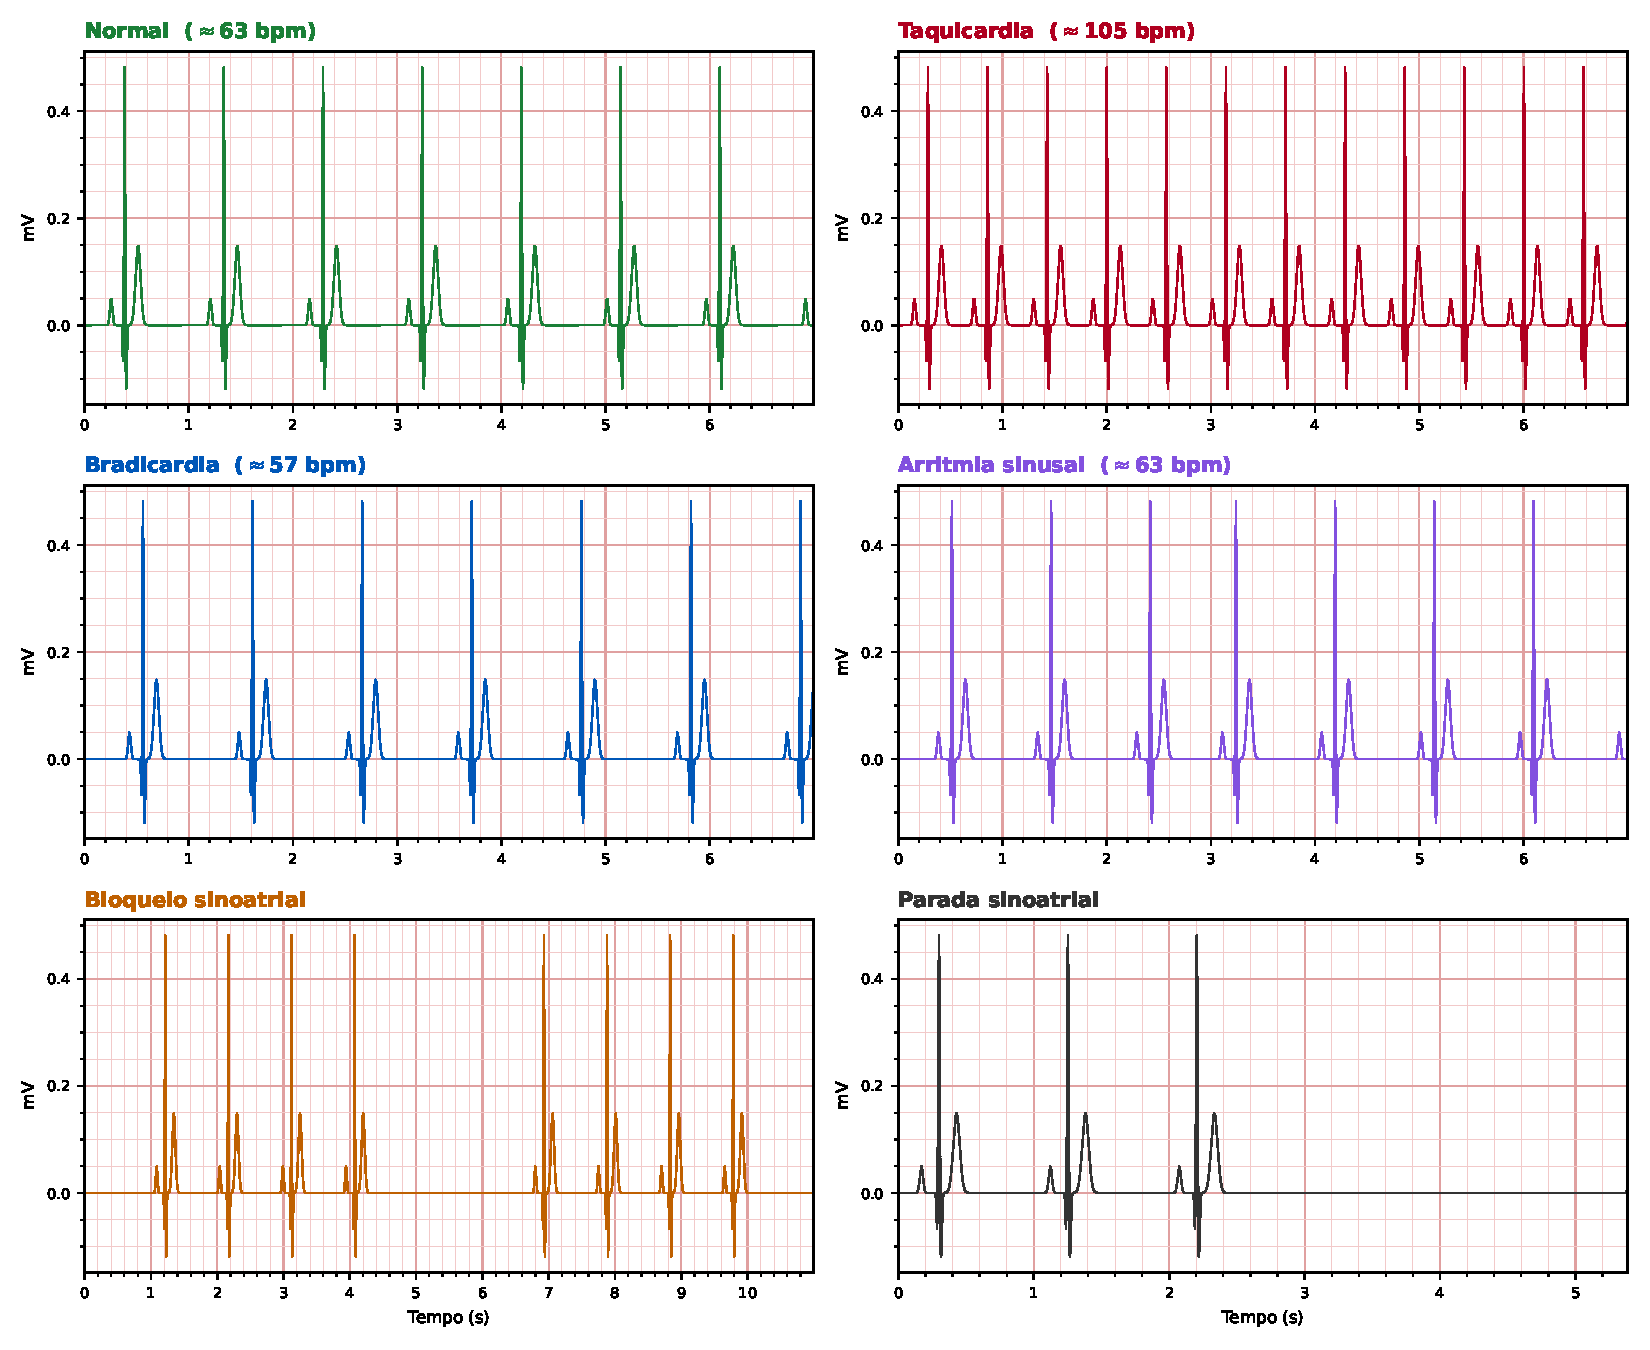
\includegraphics[width=\linewidth]{assets/casos_6classes.pdf}
\caption{Exemplos das seis classes de \acs{ECG} empregadas nos ensaios da configuração final, reproduzidos pelo gerador NI myDAQ e apresentados na escala de amplitude medida na entrada do \acs{AFE}. No painel de bloqueio a janela é centrada na pausa --- de 3,00 vezes o intervalo R-R mediano, equivalente à ausência de dois complexos QRS ---, de modo que se observe a retomada do ritmo; no de parada, a janela mostra primeiro os batimentos e termina dentro da pausa, de 3,50 vezes o intervalo mediano.}
\label{fig:casos6classes}
\end{figure}

\subsection{Desempenho sobre ECG sem ruído}
\label{sec:resFinalLimpo}

Antes de comprometer as horas de bancada, verificou-se que o binário gravado no dispositivo era de fato o que contém a sexta classe. Empregou-se, para isso, um \acs{ECG} discriminante: uma pausa de 2,2 vezes o intervalo R-R, que recai na descontinuidade identificada na Seção~\ref{sec:resZonaMorta} e que, portanto, a versão anterior classificaria como normal. A coleta retornou a máscara \texttt{0x22} --- anomalia não caracterizada acompanhada de bradicardia, esta última porque a pausa desloca a frequência média ---, confirmando a versão em execução. O procedimento é registrado por constituir a única forma de distinguir as duas versões do \textit{firmware} a partir de sua saída.

Os ensaios conduzidos sobre a configuração assim confirmada classificaram corretamente os 180 segmentos (Tabela~\ref{tab:matrizBat13}). Cada \acs{ECG} acendeu exclusivamente a sua própria \textit{flag}, e em nenhum dos 180 segmentos a sexta classe foi ativada. Esta segunda observação tem peso equivalente ao da taxa de acerto: uma classe destinada ao que não se enquadra, se disparasse sobre sinal limpo de classe conhecida, constituiria defeito, não cobertura.

\begin{table}[htb]
\centering
\caption{Matriz de confusão da configuração final sobre \acs{ECG} sem ruído (30 segmentos por classe).}
\label{tab:matrizBat13}
\resizebox{\textwidth}{!}{%
\begin{tabular}{lrrrrrrr}
\hline
\textbf{Classe do \acs{ECG}} & \textbf{Normal} & \textbf{Taqui.} & \textbf{Bradi.} & \textbf{Arritmia} & \textbf{Bloqueio} & \textbf{Parada} & \textbf{Não caract.} \\
\hline
Normal              & 30 & 0 & 0 & 0 & 0 & 0 & 0 \\
Taquicardia         & 0 & 30 & 0 & 0 & 0 & 0 & 0 \\
Bradicardia         & 0 & 0 & 30 & 0 & 0 & 0 & 0 \\
Arritmia sinusal    & 0 & 0 & 0 & 30 & 0 & 0 & 0 \\
Bloqueio sinoatrial & 0 & 0 & 0 & 0 & 30 & 0 & 0 \\
Parada sinoatrial   & 0 & 0 & 0 & 0 & 0 & 30 & 0 \\
\hline
\end{tabular}%
}
\end{table}

Valem aqui, integralmente, as ressalvas já registradas: o \acs{ECG} cedido é exatamente periódico e seus ritmos foram deliberadamente afastados dos limiares de decisão, de modo que o resultado estabelece que o sistema não erra sobre sinal controlado, e não que acerte sobre \acs{ECG} arbitrário. A medida pertinente para esta última pretensão é a da base MIT-BIH (Seção~\ref{sec:resMITBIH}).

\subsection{Desempenho sob ruído somado}
\label{sec:resFinalRuido}

As mesmas seis classes foram submetidas às três formas de ruído especificadas na
Seção~\ref{sec:resRuido}, cada uma em três amplitudes, perfazendo 54 condições e 1.620
ensaios. A taxa de acerto total foi de 92,6\,\% (1.500 de 1.620), sem qualquer erro de
processamento. A Tabela~\ref{tab:ruidoFinal} discrimina o desempenho por condição e por
classe.

\begin{table}[htb]
\centering
\caption{Desempenho da configuração final por condição de ruído (30 segmentos por classe; 180 ensaios por condição). A última coluna traz o erro absoluto médio de estimativa da frequência cardíaca.}
\label{tab:ruidoFinal}
\resizebox{\textwidth}{!}{%
\begin{tabular}{lrrrrrrrr}
\hline
\textbf{Condição} & \textbf{Normal} & \textbf{Taqui.} & \textbf{Bradi.} & \textbf{Arritmia} & \textbf{Bloqueio} & \textbf{Parada} & \textbf{Total} & \textbf{MAE FC (bpm)} \\
\hline
Deriva 0,33 Hz, 10\,\% & 30/30 & 30/30 & 30/30 & 30/30 & 30/30 & 30/30 & 180/180 & 0,2 \\
Deriva 0,33 Hz, 20\,\% & 30/30 & 30/30 & 30/30 & 30/30 & 30/30 & 30/30 & 180/180 & 0,2 \\
Deriva 0,33 Hz, 30\,\% & 30/30 & 30/30 & 30/30 & 30/30 & 30/30 & 30/30 & 180/180 & 0,2 \\
Rede 60 Hz, 10\,\%     & 30/30 & 30/30 & 30/30 & 30/30 & 30/30 & 30/30 & 180/180 & 0,2 \\
Rede 60 Hz, 20\,\%     & 30/30 & 30/30 & 30/30 & 30/30 & 30/30 & 30/30 & 180/180 & 0,3 \\
Rede 60 Hz, 30\,\%     & 0/30  & 0/30  & 0/30  & 0/30  & 30/30 & 30/30 & 60/180  & 14,1 \\
Aleatório, 10\,\%      & 30/30 & 30/30 & 30/30 & 30/30 & 30/30 & 30/30 & 180/180 & 0,2 \\
Aleatório, 20\,\%      & 30/30 & 30/30 & 30/30 & 30/30 & 30/30 & 30/30 & 180/180 & 0,2 \\
Aleatório, 30\,\%      & 30/30 & 30/30 & 30/30 & 30/30 & 30/30 & 30/30 & 180/180 & 0,2 \\
\hline
\textbf{Global}        &       &       &       &       &       &       & \textbf{1.500/1.620} & \\
\hline
\end{tabular}%
}
\end{table}

Oito das nove condições resultaram em taxa de acerto integral, com erro de estimativa da
frequência cardíaca inferior a 0,3~bpm. A deriva de linha de base foi rejeitada até a
amplitude máxima, resultado atribuível ao filtro passa-altas de 0,5~Hz, cuja frequência de
corte situa-se acima da componente de 0,33~Hz da perturbação. O ruído aleatório de banda
larga, que atravessa parcialmente a cascata de filtros e poderia produzir picos indesejados,
também não degradou o desempenho em nenhuma amplitude --- diferentemente do que se observara
sob a versão original do algoritmo (Seção~\ref{sec:resRuido}), em que a maior amplitude
custava parte dos segmentos normais.

A totalidade das 120 falhas concentra-se na interferência de rede de 60~Hz na amplitude de
30\,\%, e o modo de falha difere daquele observado sob a versão original. Sob essa condição,
as quatro classes definidas pelo ritmo foram classificadas como \textbf{bloqueio
sinoatrial}, enquanto o bloqueio e a parada permaneceram corretos. O mecanismo subjacente é o
mesmo já caracterizado --- a perda de picos R ---, mas sua consequência mudou com o critério
de pausa: um pico não localizado produz um intervalo R-R de exatamente duas vezes a mediana
do segmento, que é precisamente a definição de bloqueio na formulação relativa
(Seção~\ref{sec:resCriterioPausa}). O erro absoluto médio de estimativa da frequência
cardíaca nessa condição, de 14,1~bpm contra menos de 0,3~bpm nas demais, quantifica a
extensão da perda.

Convém estabelecer onde, na cadeia, essa perda ocorre --- questão que a taxa de acerto por si só não responde. Para dirimi-la, gravou-se no dispositivo o conteúdo do \textit{buffer} de detecção, isto é, a sequência de amostras que o algoritmo efetivamente recebeu após o divisor resistivo, o \acs{AFE} e os filtros digitais, e transferiu-se esse traçado pela interface serial (Apêndice~\ref{ap:figurasRuido}, Figura~\ref{fig:rawAdquirido}). O resultado é inequívoco: os complexos QRS encontram-se \textbf{íntegros} no sinal adquirido, com ritmo regular --- um detector de limiar simples localiza todos eles, e o intervalo R-R mediano permanece em 952~ms, idêntico ao do \acs{ECG} sem perturbação. A perda não é, portanto, da aquisição. Ela ocorre na \emph{localização} dos picos: o algoritmo de detecção reconheceu 27 dos 32 complexos presentes, e o intervalo resultante de 1.908~ms satisfez o critério de bloqueio.

A observação é coerente com o método empregado na detecção. O algoritmo reaproveitado localiza os complexos pelo método da operação de diferenças (Seção~\ref{sec:deteccaoBorda}), que opera sobre a \emph{derivada} do sinal e pareia máximos com mínimos locais. Uma interferência senoidal de 60~Hz possui derivada da mesma ordem de grandeza que a do complexo QRS, de modo que o pareamento de extremos se desorganiza e o limiar adaptativo se desloca. Corrobora essa leitura o comportamento sob ruído aleatório de idêntica amplitude, que não produz o efeito (Tabela~\ref{tab:ruidoFinal}): não é a energia da perturbação que compromete a detecção, mas sua periodicidade. Trata-se, pois, de limitação do algoritmo de detecção de picos, e não da cadeia de aquisição desenvolvida neste trabalho. Sob o critério absoluto anterior, o mesmo intervalo --- de aproximadamente 2~s, para um ritmo de 1~s --- não alcançava o piso de 4~s e não era interpretado como pausa; a versão original registrava, nessa condição, deslocamento da frequência cardíaca estimada, e não detecção de pausa. A bradicardia, que ali permanecia correta por continuar acima do limiar de 1000~ms mesmo com a frequência subestimada, passa agora a ser suprimida pela pausa indevida. O erro absoluto médio de estimativa da frequência cardíaca nessa condição, de 14,0~bpm contra menos de 0,3~bpm nas demais, quantifica a extensão da perda de picos.

Convém delimitar, por fim, o que a sexta classe de anormalidade \emph{não} resolve. Sob esta
condição ela não altera a classificação: a perda de picos é sistemática e produz intervalos
de exatamente duas vezes a mediana, que \emph{satisfazem} o critério de bloqueio. Não há, aqui,
uma lacuna entre critérios a preencher --- há um critério sendo satisfeito pela razão errada.
A classe acrescenta, ainda assim, informação ao registro: os segmentos de arritmia sinusal e
de bloqueio passam a apresentar a máscara \texttt{0x28}, registrando que, além do bloqueio
aparente, havia no segmento intervalos não enquadráveis em nenhum critério --- indício da
anomalia de aquisição que a versão anterior descartava, útil à inspeção posterior do traçado.
Os traçados das seis classes sob essa condição, o detalhe da interferência sobre o complexo
QRS e a série de intervalos R-R dela resultante são reunidos no
Apêndice~\ref{ap:figurasRuido}.

Consolidando os dois conjuntos de ensaios desta seção, registram-se 1.800 segmentos coletados, correspondentes a 15,0 horas de \acs{ECG} e a 34,6 milhões de amostras processadas, com 58.787 picos R detectados, \textbf{sem um único erro de aquisição}. O erro absoluto médio de estimativa da frequência cardíaca, excluída a condição de rede a 30\,\%, foi de 0,19~bpm sobre 1.620 segmentos.

Esses dados respondem afirmativamente à primeira das duas perguntas formuladas na Seção~\ref{sec:validacaoGerador}: a anomalia foi corretamente identificada e codificada no \textit{payload}. Em cada um dos 1.800 ensaios registrou-se, além da classe detectada, o \textit{payload} de 10 bytes montado pelo \textit{firmware}, tal como seria transmitido. Submetidos à mesma função decodificadora cadastrada no \textit{ChirpStack} (Seção~\ref{sec:resPipeline}) e confrontados campo a campo com a saída do detector, os 1.800 \textit{payloads} mostraram-se corretos --- máscara de anomalias, frequência cardíaca, intervalo R-R médio e seu desvio, contagem de picos e identificador de segmento, sem uma única divergência. A codificação do resultado da detecção, portanto, não introduz erro: o desempenho do sistema na identificação da anomalia é o da classificação, reportado nas seções anteriores, e nada se perde entre ela e a montagem do quadro a transmitir.

Quanto à segunda pergunta, o evento correto chegou ao aplicativo, conforme verificado na Seção~\ref{sec:resPipeline}. Essa verificação foi conduzida à parte dos ensaios de classificação, pela razão ali exposta: o protocolo de disparo único exige que o processamento do segmento seja iniciado por comando, o que impôs manter o enlace de rádio desativado durante os ensaios. Confrontando-se o \textit{payload} publicado com o evento persistido no banco e exibido no aplicativo, verificou-se a correspondência para as seis classes. Reconhece-se, contudo, que essa verificação tem alcance menor que a das baterias: apoia-se em seis \textit{uplinks} representativos, e não em repetição estatística. A validação conjunta do enlace de rádio com a aquisição, em regime contínuo, permanece como etapa subsequente (Capítulo~\ref{chap:conclusoes}).

Estes números caracterizam a cadeia de aquisição e de codificação desenvolvida nesta dissertação, distintamente do desempenho do algoritmo de detecção nela embarcado.

\section{Ensaios com ECG Real de Banco Público}
\label{sec:resMITBIH}

Todos os ensaios anteriores se apoiaram em \acs{ECG} gerado artificialmente e medem, por isso, o desempenho do sistema sobre morfologias e ritmos controlados. Para verificar se o desempenho observado se sustenta sobre o \acs{ECG} de pacientes reais, com toda a variabilidade fisiológica que o \acs{ECG} sintético não reproduz, recorreu-se à base MIT-BIH de arritmias — repositório público anotado por cardiologistas, de referência consolidada na literatura. Dela extraíram-se 60 segmentos de 30~s, 15 para cada uma de quatro classes — normal, taquicardia, bradicardia e arritmia sinusal —, classificadas por seus intervalos R-R. As duas classes de pausa ficaram de fora desta etapa. A seleção partiu de dezoito registros, escolhidos por cobrirem, em conjunto, as quatro classes acima, e em nenhum deles ocorre pausa na faixa exigida pelo critério de detecção. Selecionar registros pelas classes de pausa, por sua vez, não é possível de forma direta: as anotações de ritmo do MIT-BIH não preveem bloqueio nem parada sinoatrial --- o único bloqueio anotado na base é o atrioventricular de segundo grau, presente em um único registro ---, de modo que localizá-las exige varrer os intervalos R-R registro a registro. Essa varredura foi conduzida em seguida e é relatada adiante: ela recuperou o bloqueio, em um registro fora da seleção inicial, e confirmou a indisponibilidade da parada sinoatrial.

\subsection{Desempenho do algoritmo isolado}
\label{sec:resMitbihAlgoritmo}

Numa primeira etapa, os 60 segmentos foram fornecidos diretamente ao algoritmo de detecção, sem passar pela cadeia de aquisição, de modo a medir o \emph{algoritmo} isoladamente sobre o sinal real. A taxa de acerto total foi de 81,7\,\% (49 dos 60 segmentos), com a matriz de confusão da Tabela~\ref{tab:matrizMITBIH}. A queda em relação aos 100\,\% dos ensaios com \acs{ECG} controlado concentra-se, quase integralmente, no critério de arritmia sinusal: das onze classificações incorretas, dez são detecções de arritmia sobre segmentos de outras classes, e seu valor preditivo positivo cai a 58\,\%. Trata-se da mesma baixa especificidade caracterizada na Seção~\ref{sec:resArritmia}, agora manifesta sobre \acs{ECG} real: a variabilidade batimento a batimento naturalmente presente no ritmo de pacientes reais satisfaz o critério de arritmia sinusal, ausente do \acs{ECG} sintético regular. Esse valor de 81,7\,\% representa, assim, o teto do \emph{método} sobre sinal real, e não uma limitação introduzida pelo sistema aqui desenvolvido.

\begin{table}[htb]
\centering
\caption{Matriz de confusão sobre o \acs{ECG} real (60 segmentos do MIT-BIH, 15 por classe, fornecidos diretamente ao detector; linha = classe esperada, coluna = classe detectada).}
\label{tab:matrizMITBIH}
\begin{tabular}{l c c c c}
\hline
\textbf{Esperada / Detectada} & \textbf{Normal} & \textbf{Taqui.} & \textbf{Bradi.} & \textbf{Arrit.} \\
\hline
Normal            & 11 & 0  & 0  & 4  \\
Taquicardia       & 0  & 11 & 0  & 4  \\
Bradicardia       & 0  & 0  & 13 & 2  \\
Arritmia sinusal  & 0  & 1  & 0  & 14 \\
\hline
\end{tabular}
\end{table}

\subsection{Desempenho da cadeia completa}
\label{sec:resMitbihCadeia}

Numa segunda etapa, os mesmos segmentos do MIT-BIH foram reproduzidos pelo gerador e adquiridos pela cadeia de aquisição completa — divisor resistivo, \acs{AFE}, filtros digitais e quantização a 640~SPS —, no mesmo protocolo de disparo único das baterias anteriores. Acrescentou-se, nesta etapa, uma quinta classe. A varredura por pausas anunciada acima, estendida a registros fora da seleção inicial, localizou o registro~232. Trata-se de registro anotado como bradicardia sinusal --- manifestação da disfunção do nó sinusal, que é precisamente o quadro que produz o bloqueio sinoatrial ---, e nele há catorze pausas na faixa, agrupadas de modo a haver janelas de 30~s contendo mais de uma, condição que o critério exige. Dele extraíram-se os dois segmentos de bloqueio empregados nesta bateria. A parada sinusal permaneceu indisponível: os únicos intervalos superiores a seis segundos, entre os vinte registros varridos, ocorrem no registro~207, dentro de episódios de \textit{flutter} ventricular em que os batimentos não recebem marcação --- o intervalo é artefato de anotação, e não pausa sinusal, de modo que empregá-lo seria incorreto. Os representantes de cada classe foram escolhidos entre os segmentos que o detector já classificava corretamente na etapa anterior, maximizando a distância ao limiar de decisão, e cada um foi reproduzido 30 vezes, perfazendo 150 ensaios. O sistema classificou corretamente os 150, sem erro de processamento.

O valor dessa etapa não está no número em si — a seleção de representantes favoráveis o torna deliberadamente otimista e ele não deve ser lido como taxa de acerto do sistema sobre \acs{ECG} real qualquer —, mas na comparação \emph{pareada} com a primeira etapa. Como o conjunto de \acs{ECG} é o mesmo, a diferença entre as duas mede exclusivamente o que a aquisição acrescenta: nos segmentos em que o algoritmo decide corretamente sobre o sinal ideal, a cadeia de aquisição preserva a decisão integralmente, sem que o divisor, o \acs{AFE}, os filtros ou a quantização custem um único acerto. As duas etapas, em conjunto, separam a limitação do \emph{método} (os 81,7\,\% da sexta) do custo da \emph{aquisição} (nulo, pela oitava) — atribuição que nenhuma das duas, isolada, permitiria.

\subsection{Efeito das revisões do critério sobre o ECG real}
\label{sec:resMitbihConfig}

Os valores das duas etapas referem-se ao critério de pausa por duração absoluta, vigente quando foram medidas. Como a revisão desse critério altera a regra de decisão, os 60 segmentos foram reavaliados sobre as configurações posteriores do detector, e o resultado é reportado na Tabela~\ref{tab:mitbihConfig}. A formulação relativa, isoladamente, reduz a taxa de acerto a 71,7\,\%: em ritmos intrinsecamente irregulares --- fibrilação atrial e ectopia ventricular frequente, presentes nos registros 200, 202 e 203 --- a mediana deixa de representar um ritmo de base, e sete segmentos passam a satisfazer o critério de pausa sem que haja pausa sinusal. O mecanismo é o mesmo identificado na Seção~\ref{sec:resFinalRuido}: intervalos R-R longos, aqui de origem fisiológica e não de perda de picos, satisfazem a razão exigida. Com a sexta classe de anormalidade descrita na Seção~\ref{sec:resNaoCaracterizada}, que reclassifica essas pausas em vez de afirmá-las, a taxa de acerto alcança 85,0\,\%, superando o valor da configuração original.

\begin{table}[htb]
\centering
\caption{Taxa de acerto sobre os 60 segmentos do MIT-BIH nas configurações do critério de detecção. $^{\dagger}$ Configuração avaliada apenas sobre esta base, sem ensaio em bancada.}
\label{tab:mitbihConfig}
% Terceira coluna em p{}: com especificador `l` o texto não quebra e a tabela
% ultrapassa a margem da página.
\begin{tabular}{@{}l c p{6.2cm}@{}}
\hline
\textbf{Configuração do critério} & \textbf{Taxa de acerto total (\%)} & \textbf{Limitação dominante} \\
\hline
Pausa por duração absoluta    & 81,7 & Especificidade da arritmia sinusal \\
Pausa relativa ao R-R         & 71,7 & Falso positivo de pausa em ritmo irregular \\
Pausa relativa + sexta classe & 85,0 & Especificidade da arritmia sinusal \\
Limiar de ritmo pela mediana$^{\dagger}$ & 90,0 & Especificidade da arritmia sinusal \\
\hline
\end{tabular}
\end{table}


Cabe registrar, por último, uma melhoria identificada depois de concluídos os ensaios de bancada e
avaliada apenas sobre esta base, sem passar pela bancada. O critério de pausa compara a
duração do intervalo com a mediana do segmento, mas os limiares de taquicardia e de
bradicardia continuavam a ser aplicados ao intervalo R-R \emph{médio}. A diferença é
irrelevante em ritmo regular, em que média e mediana coincidem, mas não quando há pausa: um
único intervalo longo desloca a média e pode rotular como bradicardia um segmento cujo ritmo
de base é normal. Aplicando-se os dois limiares à mediana, a taxa de acerto sobre os 60
segmentos desta base passa de 85,0\,\% para 90,0\,\%, com três segmentos corrigidos e nenhum
prejudicado --- todos em registros de ritmo intrinsecamente irregular, onde a média é menos
representativa. A alteração não foi incorporada aos ensaios relatados neste capítulo, que
medem a configuração de \textit{firmware} efetivamente ensaiada em bancada; ela é registrada
aqui como aprimoramento medido e verificável, cuja validação sobre a cadeia completa fica
para etapa subsequente (Capítulo~\ref{chap:conclusoes}).


\section{Validação do Fluxo de Dados de Ponta a Ponta}
\label{sec:resPipeline}

A integração entre a infraestrutura de rede e a camada de aplicação foi validada de forma independente da aquisição do biopotencial. Utilizando uma ferramenta de publicação \acs{MQTT} para simular \textit{uplinks} do \textit{ChirpStack}, verificou-se que o serviço de ingestão (Seção~\ref{sec:ingestor}) decodificou corretamente o \textit{payload}, identificou o dispositivo pelo seu \textit{DevEUI}, gravou o evento cardíaco na coleção correspondente do \textit{Firestore} e, nos casos críticos, registrou as notificações destinadas aos profissionais de saúde. As alterações no banco propagaram-se, em tempo real, para o aplicativo móvel por meio do mecanismo de \textit{listeners} do \textit{Firestore}, confirmando o funcionamento do caminho completo de dados: dispositivo, \textit{LoRaWAN}, \textit{ChirpStack}, \acs{MQTT}, \textit{ingestor}, \textit{Firestore} e aplicativo.

Cada \textit{uplink} carregou o \textit{payload} de 10 bytes definido na Seção~\ref{sec:resTransmissao} (Tabela~\ref{tab:payload}), no qual o primeiro byte codifica, como máscara de bits, as anomalias detectadas e os demais transportam a frequência cardíaca média e campos auxiliares de contexto. Na recepção, a função decodificadora (\textit{codec}) cadastrada no \textit{ChirpStack} (Figura~\ref{fig:decoder}) reconstrói esses campos e os disponibiliza em \texttt{data.object}; a partir deles, o serviço de ingestão deriva o tipo de evento segundo uma ordem de precedência, do achado de maior para o de menor risco: parada, bloqueio, taquicardia, bradicardia, arritmia sinusal e anomalia não caracterizada, preservando no registro a máscara completa com todas as anomalias do segmento. Essa ordem não reproduz uma taxonomia normativa --- não se identificou, na literatura consultada, prioridade estabelecida para o colapso de achados simultâneos em um único rótulo ---, mas constitui decisão de projeto, ordenada pelo risco potencial de cada condição: as pausas sinusais podem evoluir para comprometimento hemodinâmico, ao passo que a arritmia sinusal é fisiológica em repouso. Seu efeito restringe-se ao rótulo exibido, uma vez que a máscara é preservada no registro e é sobre ela que operam os contadores de alarme (Seção~\ref{sec:appFunc}). A arritmia sinusal ocupa a menor prioridade por ser muitas vezes uma alteração normal causada pela respiração, como será detalhado posteriormente na (Seção~\ref{sec:resArritmia}): como sua detecção frequentemente acompanha outras detecções, mantê-la à frente mascararia eventos críticos como a taquicardia; assim, um segmento só é classificado como arritmia quando essa é a única anomalia detectada. A precedência decide, contudo, apenas o rótulo do evento: a confirmação de alarme no aplicativo (Seção~\ref{sec:appFunc}) opera sobre a máscara preservada no registro, de modo que uma arritmia sinusal detectada em conjunto com outra anomalia continua a incrementar o seu próprio contador, ainda que o evento receba o rótulo da classe mais grave. Descartar a coocorrência seria inseguro: a informação de contexto que a arritmia carrega deixaria de existir justamente nos segmentos em que há mais de uma alteração.

A validação empregou seis \textit{payloads} representativos, um para cada classe de evento, publicados no tópico de \textit{uplink} por meio de uma ferramenta de simulação. Cada caso foi publicado 30 vezes, perfazendo 180 \textit{uplinks}: uma única publicação por classe verificaria apenas a decodificação, ao passo que a repetição permite observar se o serviço deixa de processar mensagens sob publicações sucessivas. Em todas as 180, o serviço de ingestão decodificou os campos, derivou corretamente o tipo de evento e a frequência cardíaca, e persistiu o registro na coleção de eventos cardíacos do \textit{Firestore}, sem perda nem duplicação, conforme a Tabela~\ref{tab:casosPipeline}. Os eventos propagaram-se, em tempo real, para o painel de monitoramento do aplicativo (Figura~\ref{fig:telasApp}a).

\begin{table}[htb]
\centering
\caption{Casos publicados na validação do fluxo de ponta a ponta e o respectivo evento persistido no \textit{Firestore}. Cada caso foi publicado 30 vezes; todas as 180 publicações resultaram em registro gravado.}
\label{tab:casosPipeline}
\begin{tabular}{l c c c l c}
\hline
\textbf{Caso} & \textbf{\textit{flags}} & \textbf{BPM} & \textbf{Publicações} & \textbf{Evento gravado} & \textbf{Crítico} \\
\hline
Normal        & \texttt{0x00} & 72  & 30 & NORMAL       & Não \\
Taquicardia   & \texttt{0x01} & 120 & 30 & TAQUICARDIA  & Sim \\
Bradicardia   & \texttt{0x02} & 48  & 30 & BRADICARDIA  & Sim \\
Arritmia      & \texttt{0x04} & 82  & 30 & ARRITMIA     & Sim \\
Bloqueio      & \texttt{0x08} & 50  & 30 & BLOQUEIO     & Sim \\
Parada        & \texttt{0x10} & 56  & 30 & PARADA       & Sim \\
\hline
\textbf{Total} & & & \textbf{180} & & \\
\hline
\end{tabular}
\end{table}

A consistência dos dados foi conferida confrontando os registros armazenados localmente no dispositivo, obtidos por meio dos comandos de despejo pela interface serial, com os eventos persistidos no banco em nuvem, não se observando divergências nos campos transmitidos.
\section{Verificação do Aplicativo Móvel}
\label{sec:resApp}

O aplicativo foi compilado para \textit{Android} pelo serviço de compilação em nuvem da plataforma \textit{Expo} e instalado em um aparelho físico, de onde provêm as telas desta seção. A verificação incidiu sobre o que a descrição funcional (Seção~\ref{sec:appFunc}) não determina: o comportamento da interface diante dos eventos efetivamente produzidos pela cadeia de aquisição e transmissão.

O painel de eventos cardíacos foi observado durante as publicações relatadas na Seção~\ref{sec:resPipeline}. Os eventos apareceram na lista sem qualquer recarga manual, identificados pelo tipo de anomalia, pela frequência cardíaca, pelo paciente associado e pelo horário de registro, com realce cromático proporcional à gravidade (Figura~\ref{fig:telasApp}a). A correspondência entre o que foi publicado e o que a tela exibiu --- inclusive nos valores de frequência cardíaca de cada classe --- fecha a cadeia do dispositivo à interface. Como a leitura é feita diretamente no banco em nuvem, sem \acs{API} intermediária, o aplicativo não depende da rede local em que operam o \textit{gateway} e o serviço de ingestão.

As demais telas foram exercitadas com dados do ambiente de validação (Figura~\ref{fig:telasApp}b--f): cadastro e consulta de pacientes, vínculo e desvínculo de dispositivos, ativação de profissionais pendentes e gestão de instituições. O controle de acesso por perfil e por estado de vínculo é exercido pelas regras de segurança do \textit{Firestore} (Seção~\ref{sec:seguranca}), e não pela interface, de modo que a restrição não depende do cliente.

Duas verificações ficaram fora do alcance desta etapa: a avaliação de usabilidade com os profissionais de saúde e o ensaio com vários dispositivos transmitindo ao mesmo tempo. Ambas dependem do uso em ambiente clínico, previsto como etapa futura.

\begin{figure}[htbp]
\centering
\subfloat[Painel de eventos cardíacos]{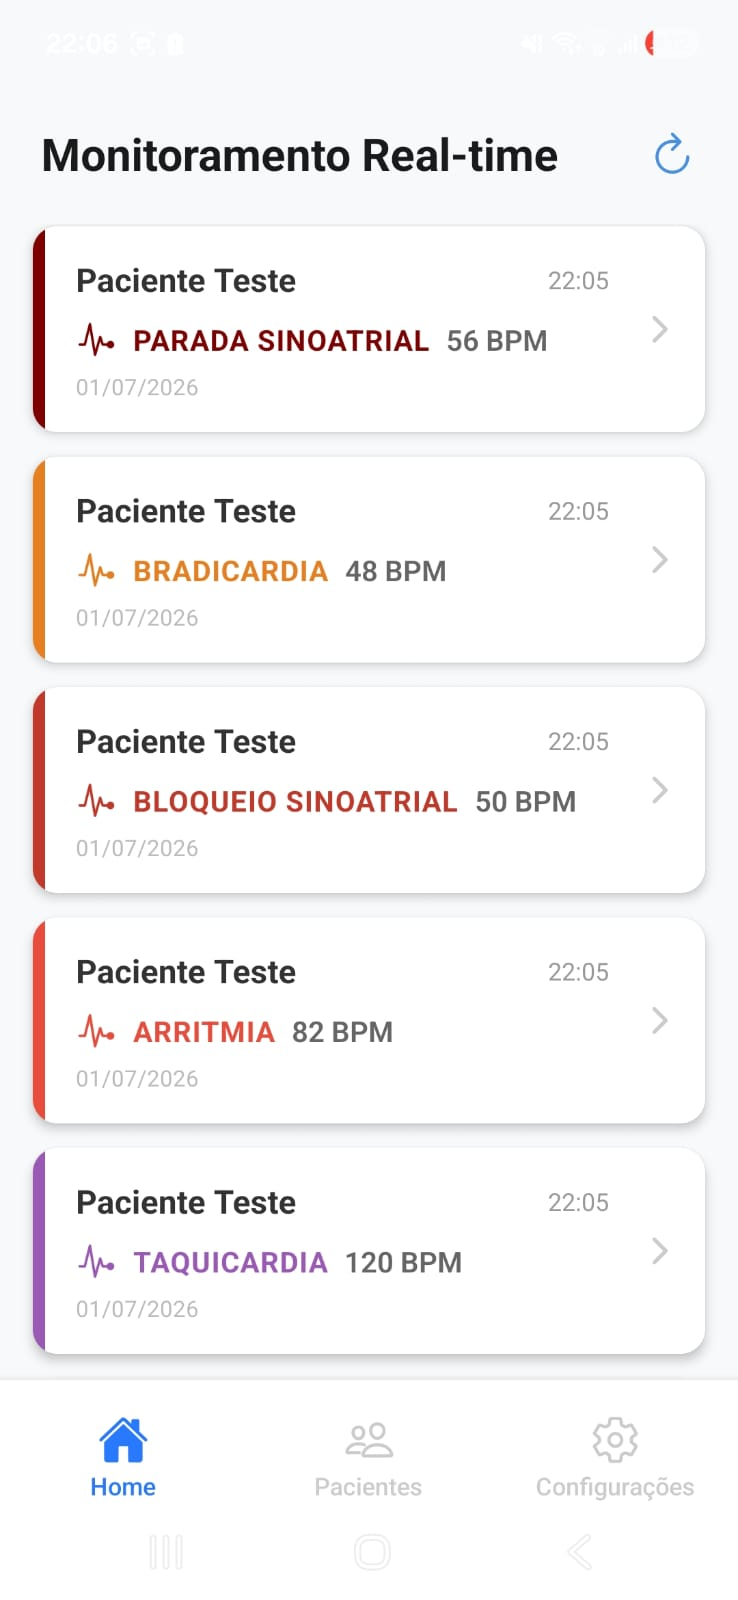
\includegraphics[width=0.30\linewidth]{assets/telaMonitoramento.jpeg}}\hfill
\subfloat[Pacientes]{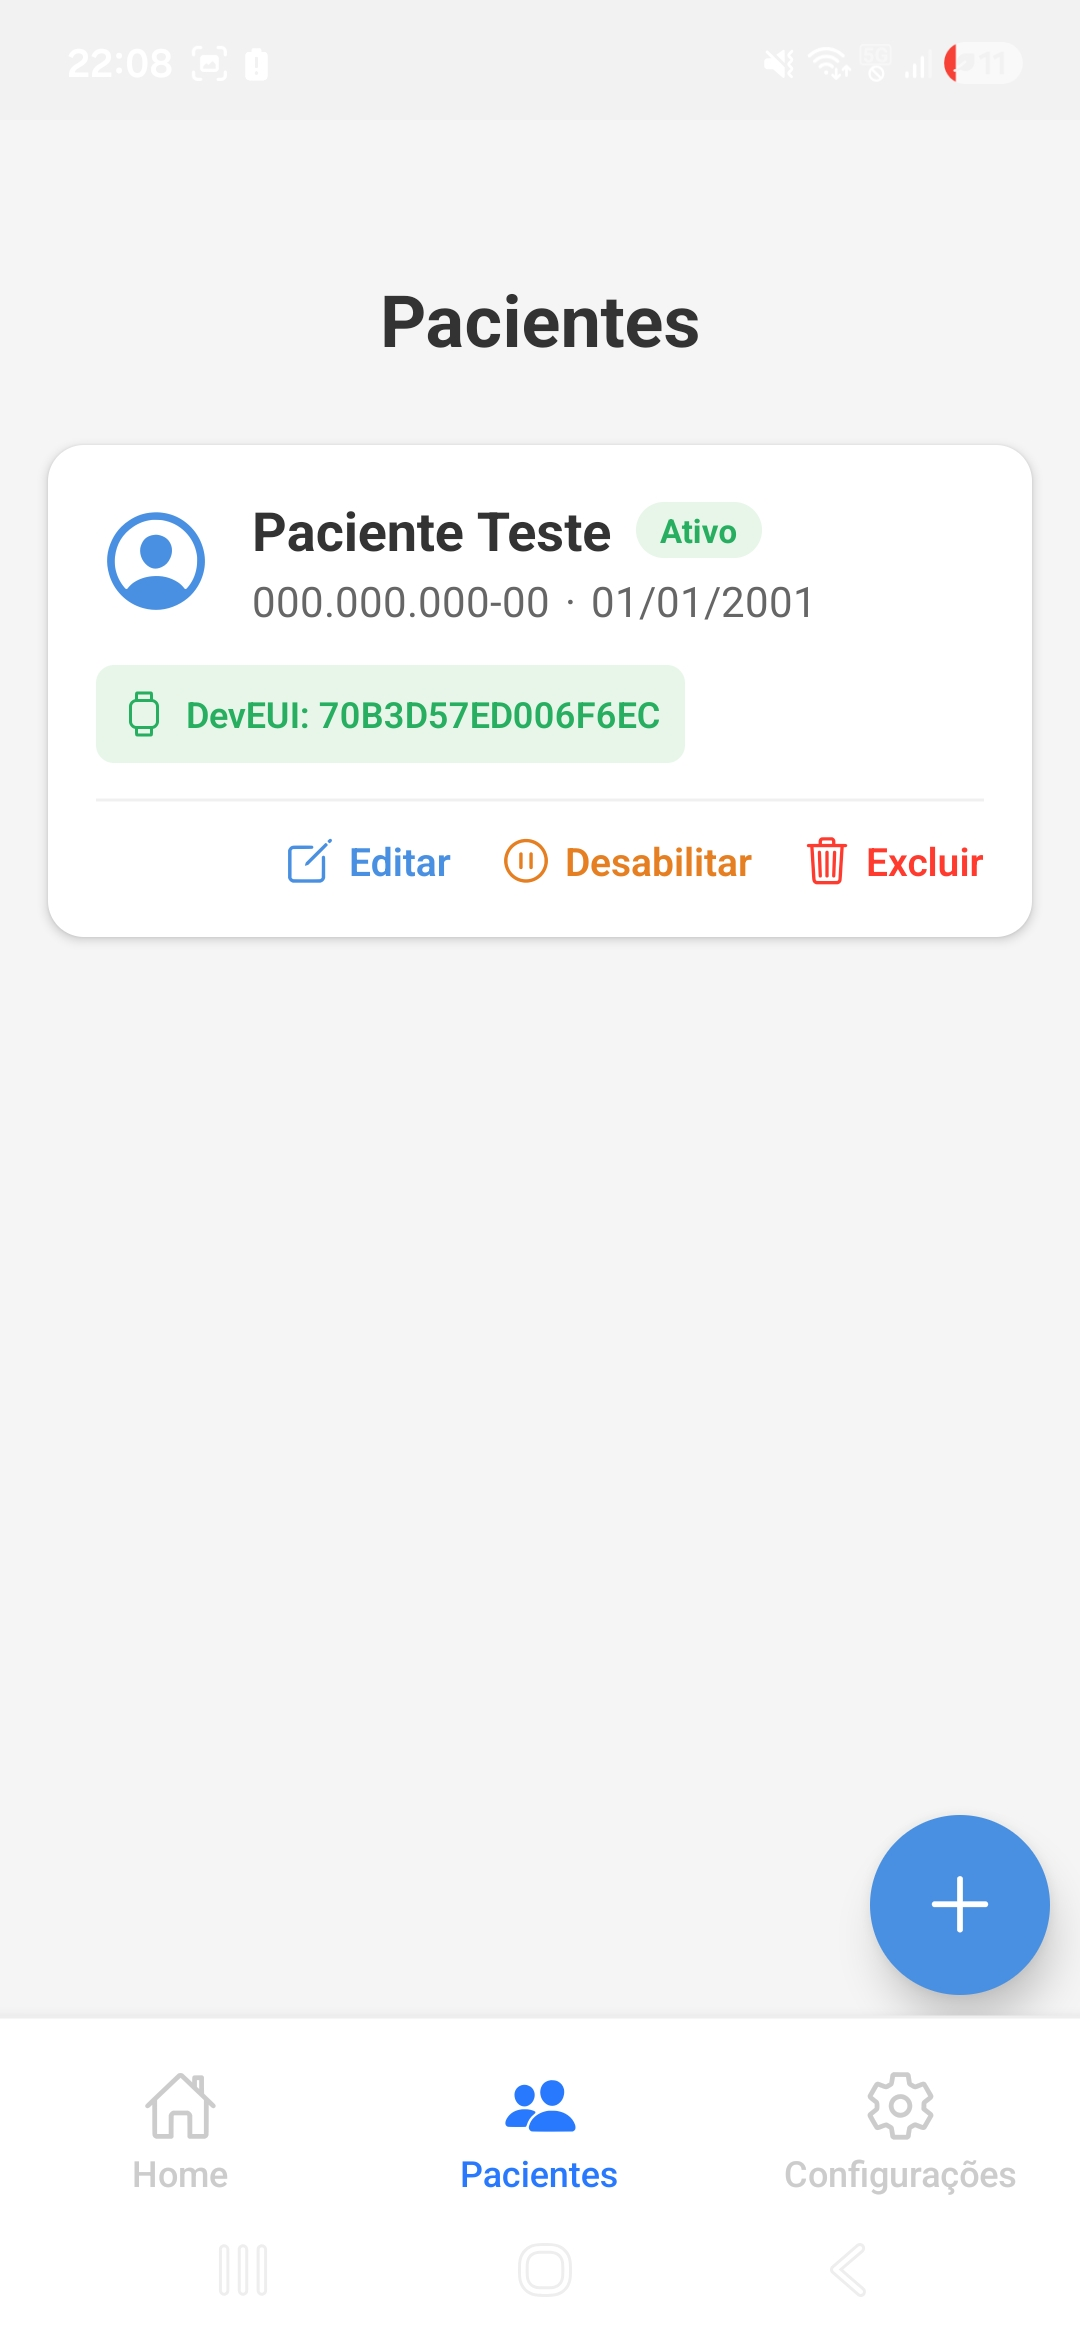
\includegraphics[width=0.30\linewidth]{assets/telaPacientes.jpeg}}\hfill
\subfloat[Dispositivos]{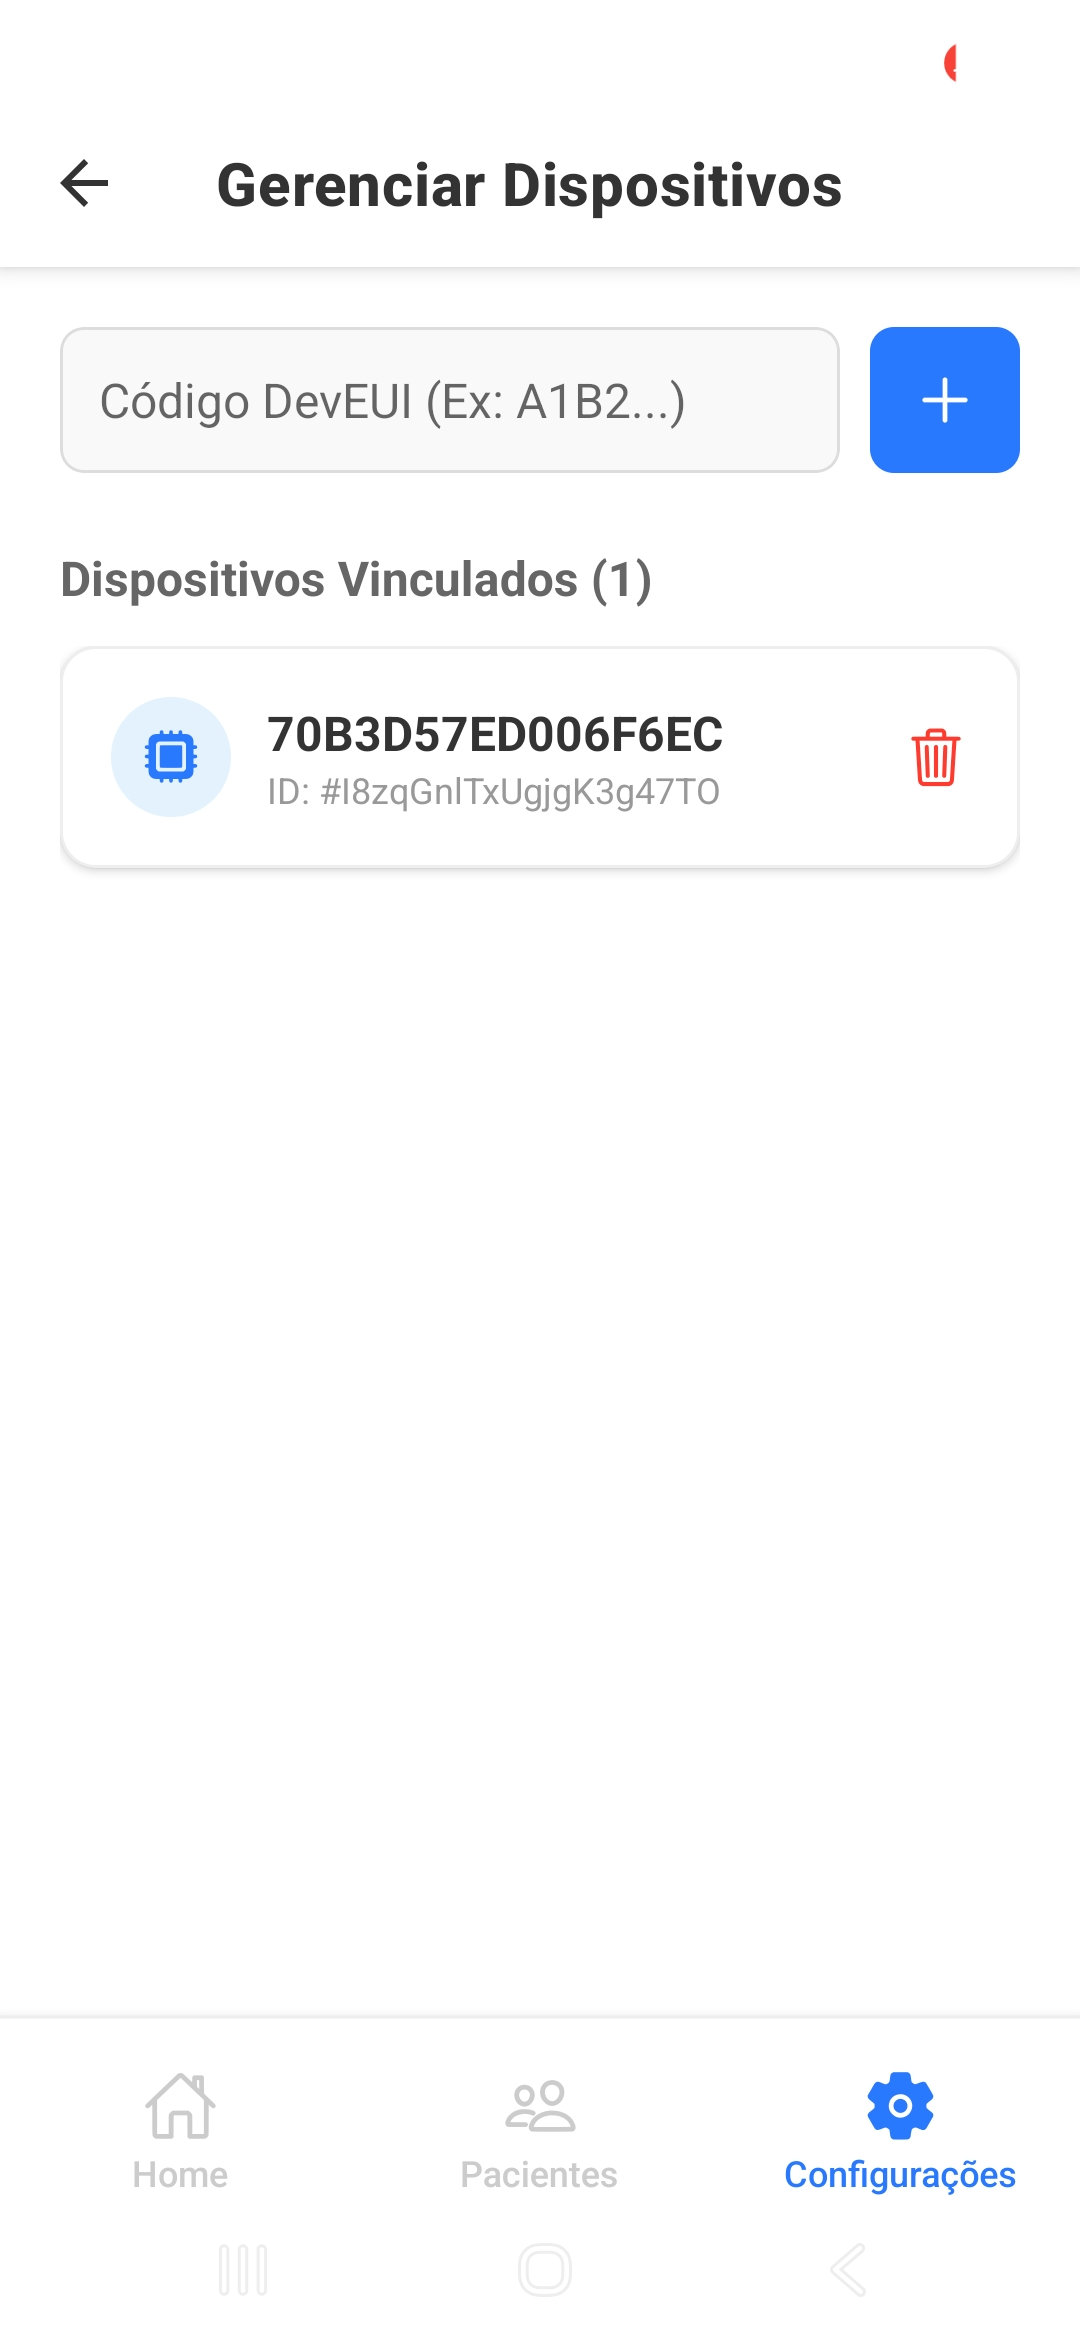
\includegraphics[width=0.30\linewidth]{assets/telaDispositivos.jpeg}}\\[1ex]
\subfloat[Usuários]{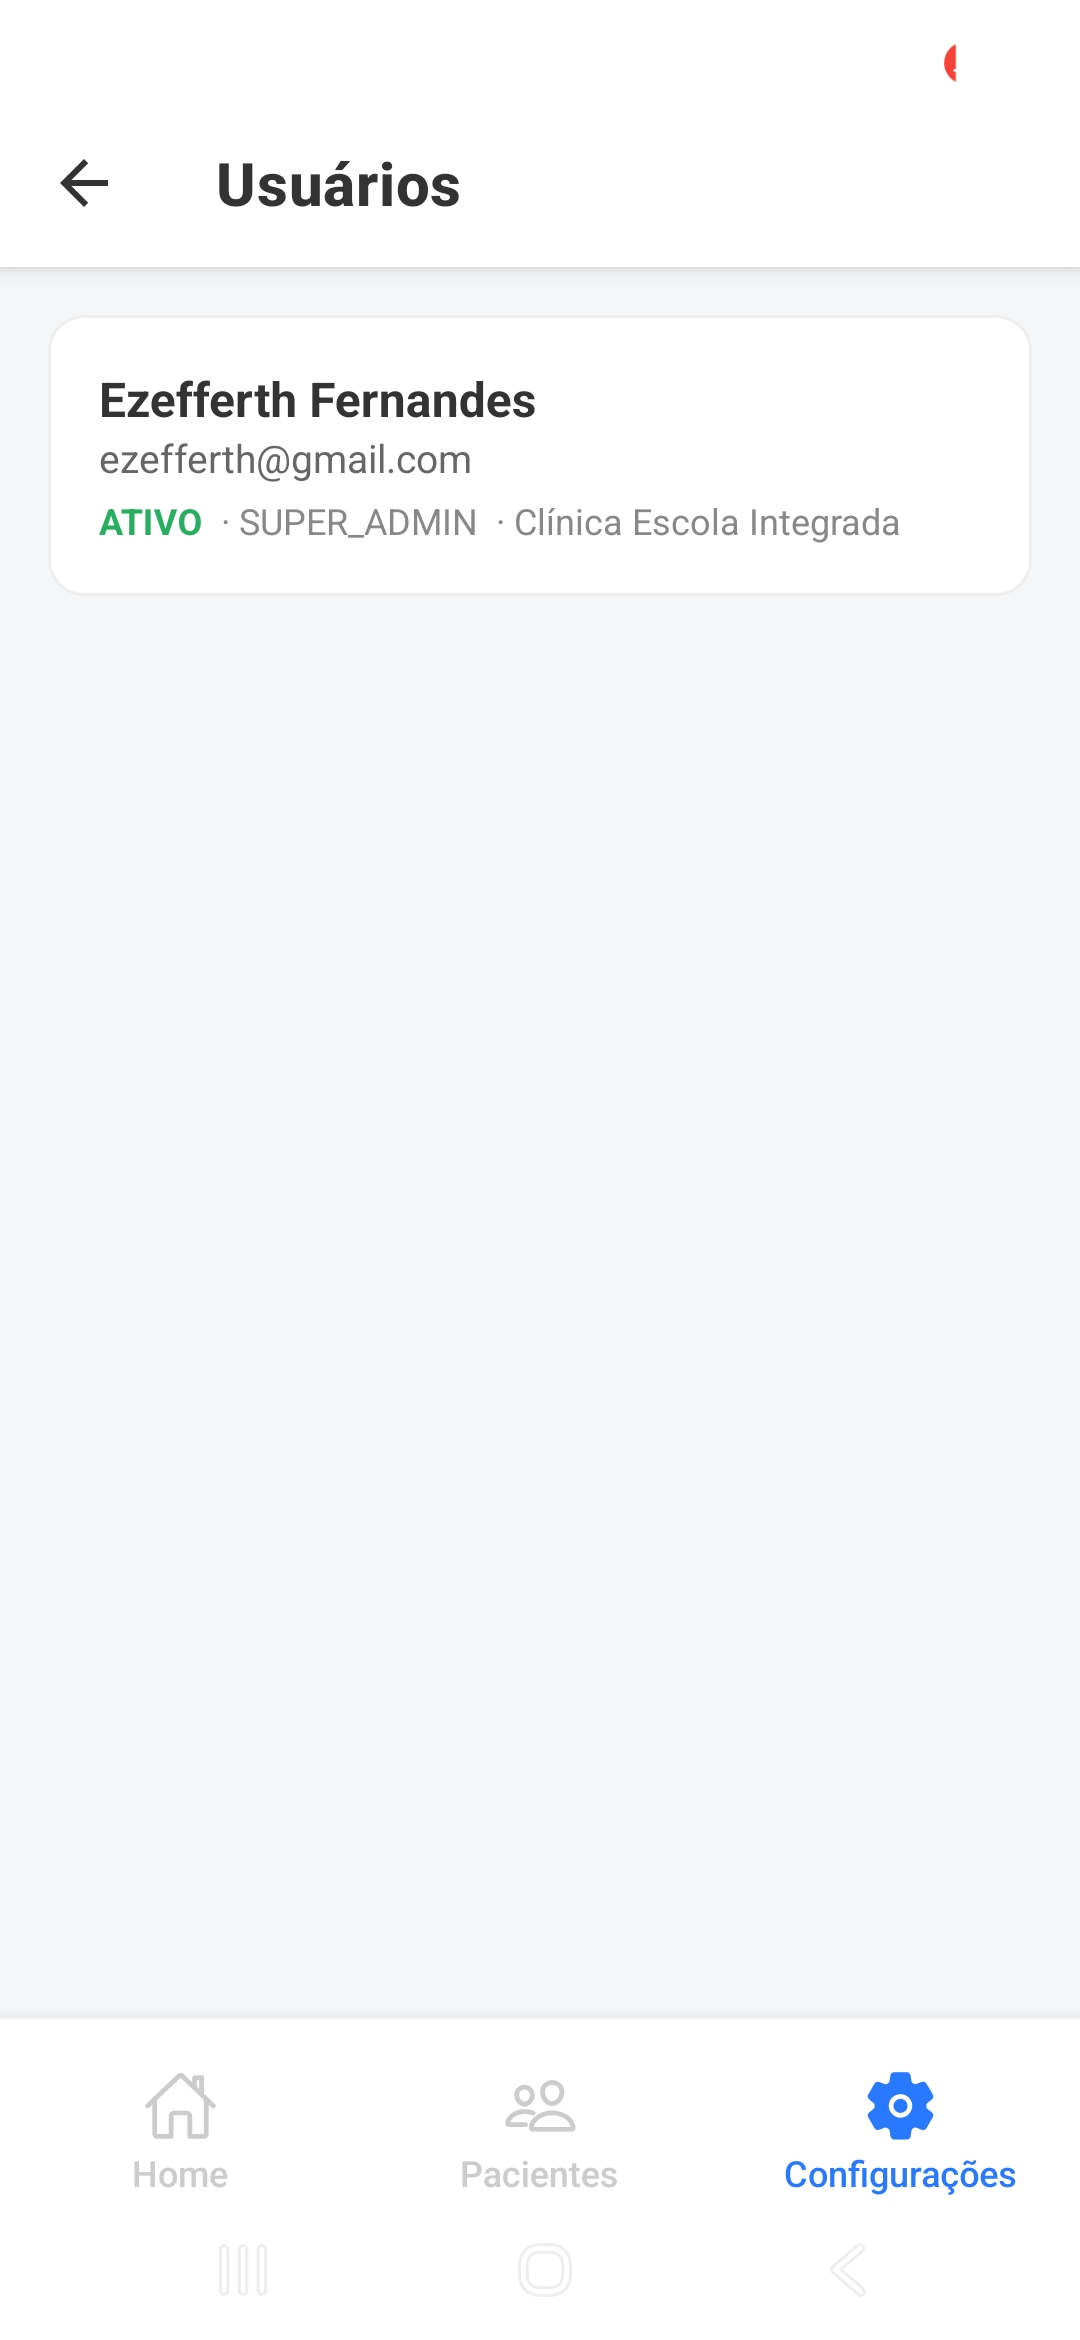
\includegraphics[width=0.30\linewidth]{assets/telaUsuarios.jpeg}}\hfill
\subfloat[Instituições]{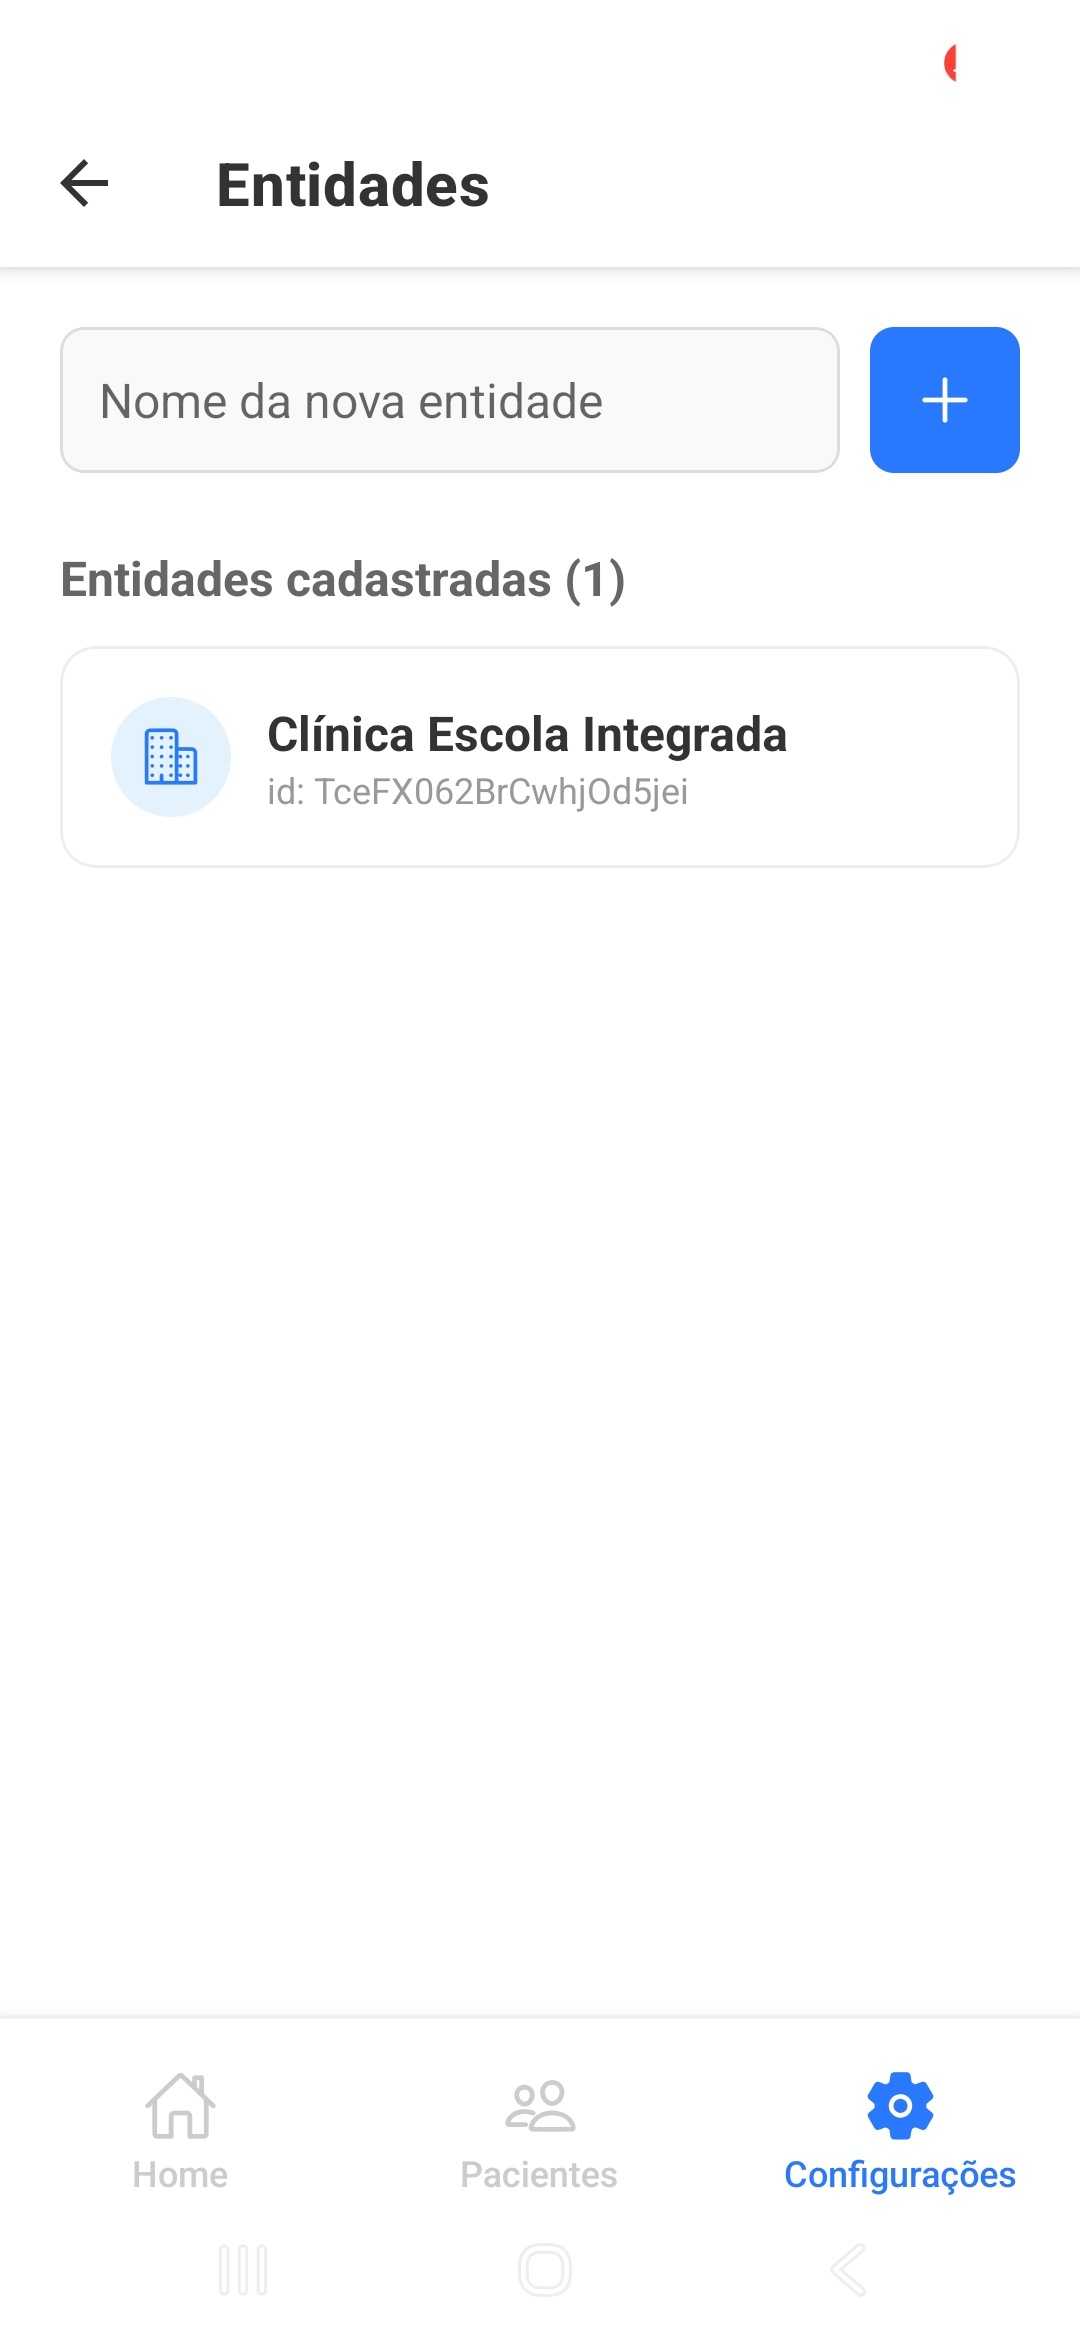
\includegraphics[width=0.30\linewidth]{assets/telaEntidades.jpeg}}\hfill
\subfloat[Configurações]{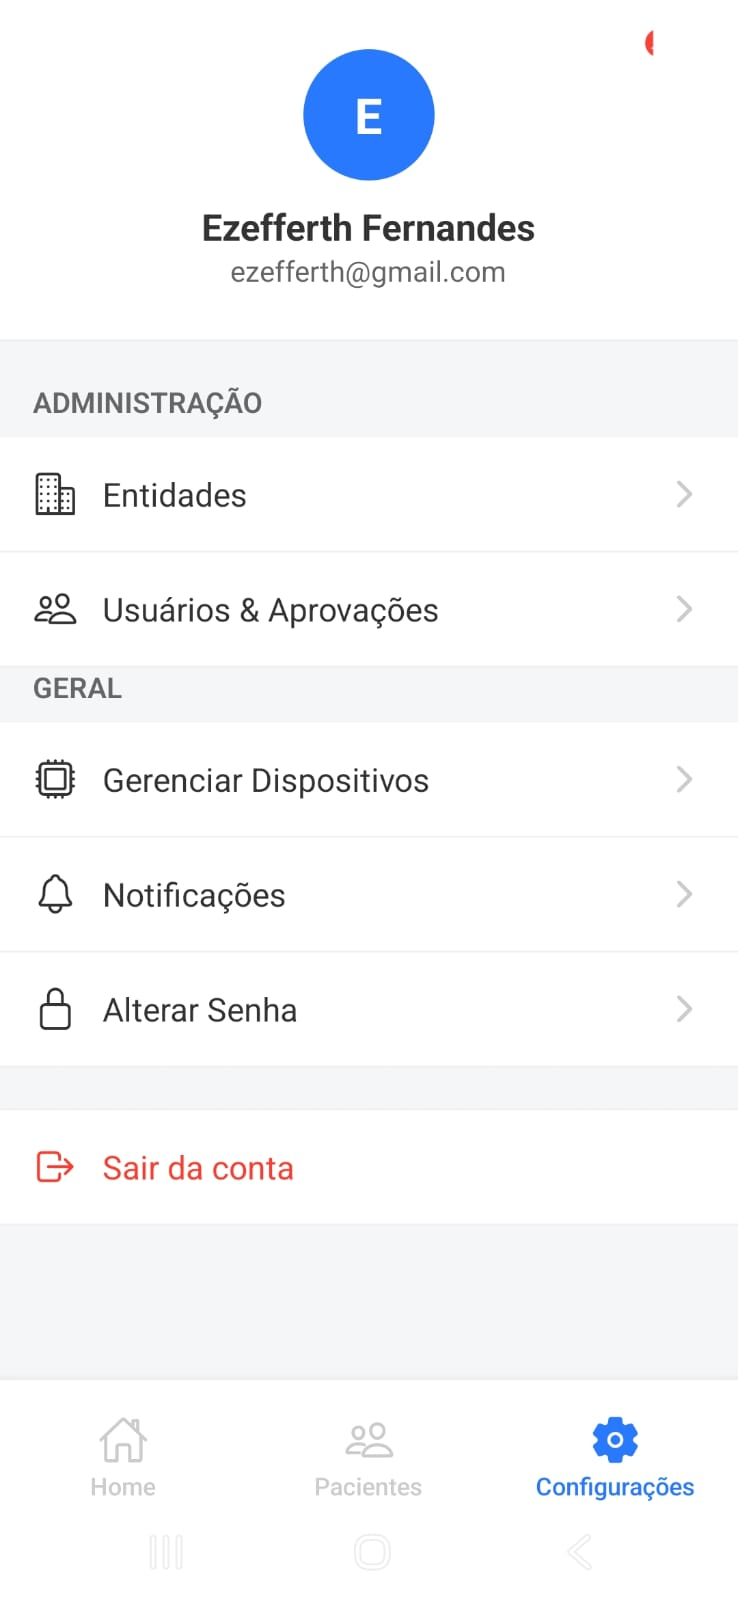
\includegraphics[width=0.30\linewidth]{assets/telaConfiguracoes.jpeg}}
\caption{Telas principais do aplicativo móvel: (a) painel de eventos cardíacos em tempo real, (b) gestão de pacientes, (c) gestão de dispositivos, (d) gestão de usuários, (e) gestão de instituições e (f) configurações.}
\label{fig:telasApp}
\end{figure}

\section{Detecção na Borda e Redução do Payload}
\label{sec:resDeteccao}

A estratégia de detecção na borda foi verificada quanto ao seu efeito sobre o volume de dados transmitidos. Enquanto a transmissão da forma de onda completa de um segmento de 30~s, à taxa efetiva de 640 SPS e 2 bytes por amostra, exigiria o envio de 38.400 bytes, o resumo produzido pelo algoritmo embarcado ocupou apenas 10 bytes por segmento — uma redução de mais de três ordens de grandeza. Esse \textit{payload} compacto é transmitido em um único \textit{uplink} a cada 30~s, com tempo de ocupação do canal (\textit{Time on Air}) reduzido e amplo respeito às restrições de \textit{duty cycle}, ao contrário da transmissão fragmentada da forma de onda, cujo tempo total inviabilizava o monitoramento contínuo (Seção~\ref{sec:resTransmissao}).

Essa abordagem é coerente com a análise de viabilidade da literatura, segundo a qual o \textit{LoRaWAN} é adequado à transmissão de alertas de detecção e de parâmetros vitais, porém não à da forma de onda contínua \citep{lorawanWaveform}. A preservação local da forma de onda dos segmentos anormais (Seção~\ref{sec:armazenamento}) manteve a possibilidade de análise detalhada \textit{a posteriori}, sem onerar o canal.
\section{Considerações sobre os Resultados}
\label{sec:resConsideracoes}

Os resultados validaram as decisões estruturais do projeto. Consolidou-se a infraestrutura
\textit{LoRaWAN} com servidor de rede local; determinou-se a taxa de amostragem efetiva do
conversor, divergente da documentada pela biblioteca de controle; corrigiu-se a aquisição do
biopotencial pela reconfiguração da referência de modo comum, obtendo-se um traçado com
morfologia adequada e ruído de rede atenuado; verificou-se a integração de ponta a ponta
entre o dispositivo, a nuvem e o aplicativo; e confirmou-se que a detecção na borda viabiliza
a operação do sistema sobre \textit{LoRaWAN}, cuja capacidade não admite a transmissão da
forma de onda.

As cinco etapas de ensaio cumpriram funções distintas, e é o conjunto delas, não qualquer uma
isolada, que sustenta as conclusões. O \acs{ECG} registrado no próprio autor
(Seção~\ref{sec:resEcgProprio}) revelou os dois defeitos de aquisição corrigidos no trabalho
--- a saturação do enlace serial e a perda periódica de amostras por bloqueio do laço --- e a
baixa especificidade do critério de arritmia sinusal em repouso. O \acs{ECG} sintetizado neste
trabalho (Seção~\ref{sec:resEcgSintetico}) estabeleceu o limite superior do desempenho, sob
ritmo controlado, e permitiu medir o erro de estimativa da frequência cardíaca na presença de
variabilidade: entre 0,2 e 0,5~bpm. O \acs{ECG} cedido pelo orientador, sob a versão original
do algoritmo (Seção~\ref{sec:resEcgOrientadorOriginal}), expôs as limitações da regra de
decisão --- em especial a definição de pausa por duração absoluta, que obrigava a adaptar o
material de teste à regra em vez de reconhecer o quadro clínico --- e a degradação sob
interferência de rede de forte amplitude. O mesmo \acs{ECG}, sob a versão final
(Seção~\ref{sec:resEcgOrientadorFinal}), mediu o efeito das revisões em condições idênticas:
classificação correta dos 180 segmentos sobre sinal sem ruído e 92,6\,\% sob as 54 condições
de ruído, com as falhas inteiramente concentradas em uma condição conhecida e diagnosticada. O
\acs{ECG} real da base MIT-BIH (Seção~\ref{sec:resMITBIH}), por fim, mediu o que nenhum sinal
sintético mede: o comportamento do método diante da variabilidade fisiológica de pacientes
reais.

Convém distinguir, nessa leitura, o que se mede sobre o \emph{algoritmo} reaproveitado do que
se mede sobre a \emph{cadeia} desenvolvida nesta dissertação. Quanto ao algoritmo, o
desempenho apresenta-se em três níveis, e é a gradação entre eles que o caracteriza: sobre
\acs{ECG} de classe conhecida e ritmo controlado não há erro de classificação; sobre \acs{ECG}
humano real, a taxa de acerto é de 85,0\,\%, limitada sobretudo pela especificidade do
critério de arritmia sinusal; e sob interferência de rede em amplitude severa o sistema falha
de modo conhecido, por perda de picos na etapa de localização dos complexos. Quanto à cadeia,
as 1.800 aquisições dos dois conjuntos de ensaios finais --- 15 horas de sinal, 34,6 milhões de amostras
--- transcorreram sem erro de aquisição, sem perda de segmento e sem uma única divergência na
montagem do \textit{payload}, com erro médio de estimativa da frequência cardíaca de
0,19~bpm. É esta última medida que responde ao objetivo desta dissertação; a primeira
caracteriza o detector reaproveitado, cuja revisão, conduzida sob orientação de seus autores,
elevou o desempenho sobre \acs{ECG} real acima do valor da formulação original.

Três limitações delimitam o alcance do que se mediu. Todo o \acs{ECG} de classe conhecida
empregado é sintético, e ainda que reproduzido fisicamente e adquirido pela cadeia completa,
não reproduz a variabilidade de morfologia de um paciente em atividade física. A única
avaliação sobre \acs{ECG} humano real foi conduzida sobre base pública, e não sobre aquisição
própria. E a entrega do evento ao aplicativo foi verificada à parte dos ensaios de classificação, sobre um
número reduzido de \textit{uplinks} representativos, porque o protocolo de disparo único exige
manter o enlace de rádio desativado. Restam, como etapas subsequentes, os ensaios clínicos
controlados com pacientes na Clínica Escola Integrada da \acs{UFMS}, a validação conjunta do
enlace de rádio com a aquisição em regime contínuo, e os ensaios de cobertura da rede e de
autonomia energética do dispositivo.
